\chapter{Gas Electron Multiplier} % (fold)
\label{cha:gas_electron_multiplier}

\section{Introduction} % (fold)
\label{sec:introduction}
The invention of Multi-Wire Proportional Chamber (MWPC) in 1968 by Georges Charpak was one of the breakthroughs in gaseous detectors, since it had better rate capability vis-a-vis its predecessors~\cite{Charpak1968}. 
This invention was also led to Nobel prize to George Charpak in 1992. With time the design and performance of MWPC have been improved. But because of our increasing demands with the acquired knowledge its limitation reached in terms of the maximum rate capability and granularity. In 1988 Anton Oed invented the Micro-Strip Gas Counter (MSGC). 
This detector had overcome the rate limitation due to positive-ion accumulation in the gas volume and able to reach up to few tens of micron in position resolution. 
Also, it can sustain the particle flux exceeding the $MHz/mm^2$ range. Its performance was very impressive but the long-term study revealed its two weakness. They are:
\begin{enumerate}
	\item Formation of deposits on the electrodes, which affects the gain and age of the detector.
	\item In presence of highly ionizing particles sometimes a destructive discharge happens.
\end{enumerate}
The invention of Micro-Pattern Gaseous Detector (MPGD) focuses these issues. 
It has unprecedented spatial resolution, large sensitive area, high rate capability, operational stability along with long lifetime, in particular, the Gas Electron Multiplier (GEM)~\cite{Sauli1997,Sauli1999,detector:1732870} detectors. 
Several new studies also showed that if a reasonable precaution has taken on the component quality it might be less vulnerable to the radiation-induced ageing than the standard silicon microstrip detectors~\cite{TITOV2004,Titov2002}.
% section introduction (end)

\section{Design and working principle of GEM} % (fold)
\label{sec:design_and_working_principle_of_gem}

GEM is a new concept from Fabio Sauli at CERN~\cite{Sauli1997}.
It is a thin plastic sheet coated with metal on both sides. It is chemically pierced by a regular array of holes using the photolithography and acid etching, as shown in Fig.~\ref{fig:gem} (left).
\begin{figure}[!htbp]
    \centering
    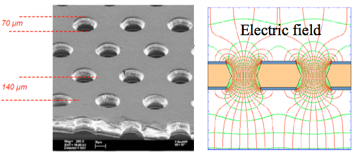
\includegraphics[width=0.95\textwidth]{figures/GEM/KEKDTP3.jpg}
    \caption{(Left) The gas electron multiplier (GEM) foil can image a two-dimensional position of particles passing through a gaseous chamber. (Right) The cross-sectional view of the GEM shows strong electric fields in the vicinity of holes where electron signals are amplified.}
    \label{fig:gem}
\end{figure}

A potential is applied betwen the two copper layers. This creates the high electric field through holes. As
\begin{equation}
    E = \frac{V}{d}
\end{equation}
where E is the electric field in GEM hole, V is the voltage applied between the two copper layers and d is the thickness of the foil. Since the Kapton\footnote{Kapton was choosen as the insulating layer as it has very good insulating power along with that it can sustain very high radiation along with that it works with wide range of temperature. It is a plastic polyimide created by DuPont.} foil is very thin, around 50 $\mu m$, so a high electric field density will be created in the hole which is shown in Fig.~\ref{fig:gem} (right).
\begin{figure}[htbp]
    \centering
    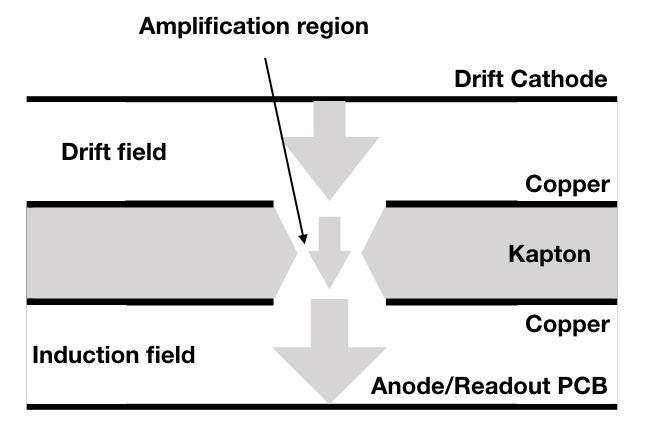
\includegraphics[width=0.75\textwidth]{figures/GEM/SingleGEM_Detector.jpeg}
    \caption{Outline of a single GEM detector.}
    \label{fig:gemOutline}
\end{figure}

The region inside the GEM detector has three different regions: drift, amplification and induction region, as shown in Fig.~\ref{fig:gemOutline}.
In the drift region, ionization occurs and electrons drift toward the GEM. 
While passing through amplification region, where few hundred volts is applied across the two copper foils, electrons gain enough kinetic energy to produce secondary ionization in the gas and starts the avalanche multiplication, as shown in Fig.~\ref{fig:gem}(right).
Finally, in the induction region, all the electrons from the amplification region reaches to the readout plane. 
If there is more than one GEM foil then through transfer region takes almost all the electrons from one GEM foil to another.

To avoid the problem of electrical breakdown a simple way is to cascade sveral GEM foils operating at lower voltages within drift cathode and the readout board.
A set of arrangement where three GEM foils are cascade is commonly known as ``\textit{Triple-GEM detector}'', as shown in Fig.~\ref{fig:gemgaps}.
\begin{figure}[!htbp]
    \begin{center}
        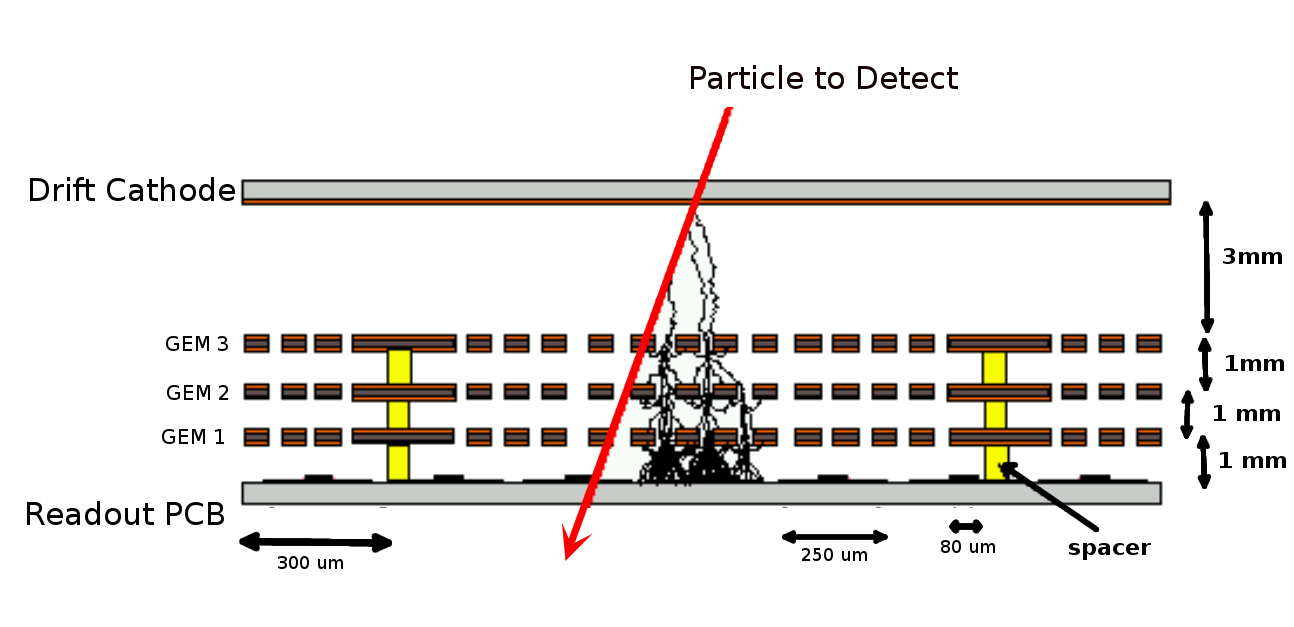
\includegraphics[width=0.95\textwidth]{figures/GEM/triple_gem.png}
        \caption{Illustration of GEM working}
        \label{fig:gemgaps}
    \end{center}
\end{figure} 

Also, the total gain is the product of the individual gain of each foil, so the gain up to $10^5$ can be achieved in this way.
In this configuration, it can reach maximum gain without any discharge or least probable.
In Fig.~\ref{fig:tripleGEM_discharge_gain} the gain and discharge probability was compared for single, double and triple GEM detectors. This shows that the triple GEM can go beyond $10^4$ gain without having any discharges.
Also, the signal readout by the electrode is pretty fast as it uses only electrons to read the signal. 
Also, using the multi-layered boards one can achieve the two-dimensional readout.
\begin{figure}[!htbp]
    \centering
    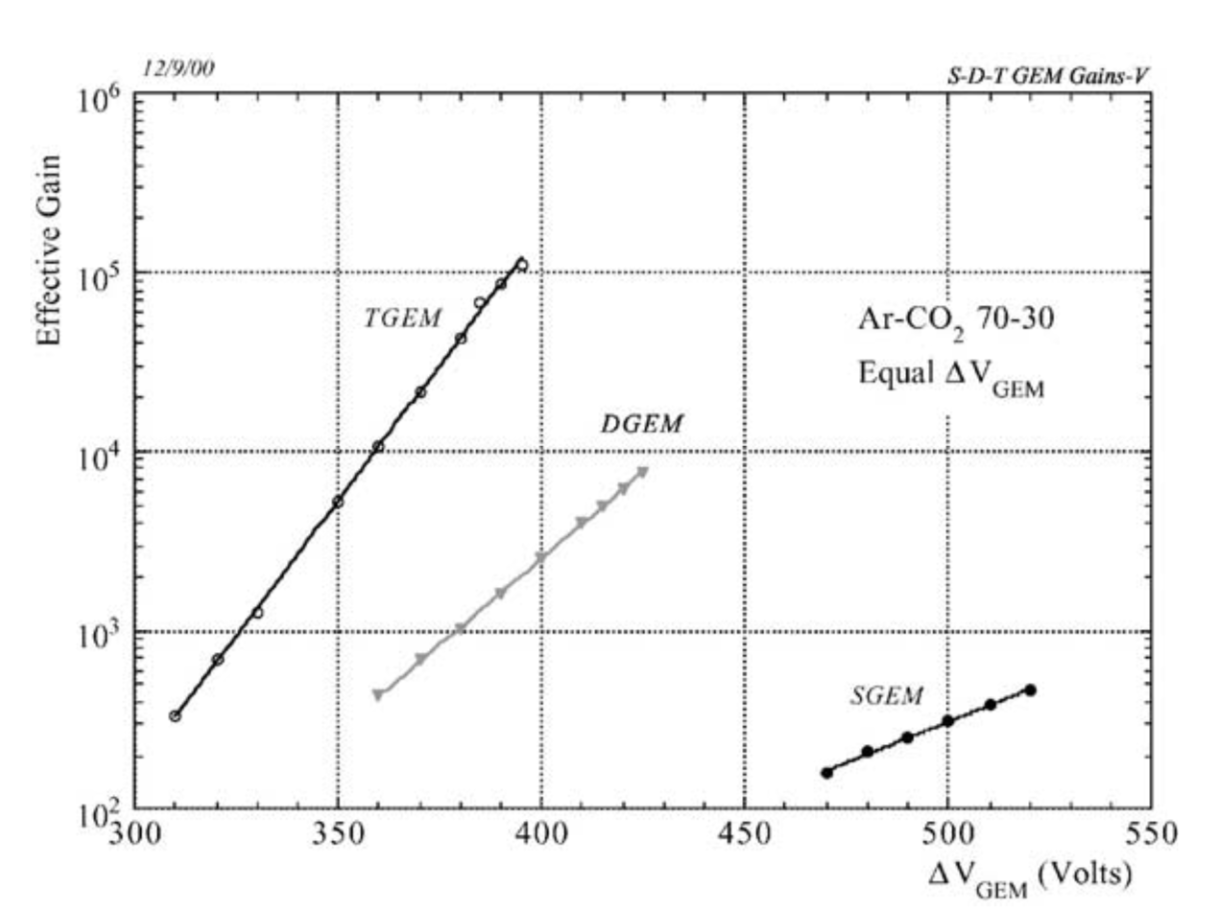
\includegraphics[width=0.45\textwidth]{figures/GEM/Comp_threeGEMS_Gain.png}%
    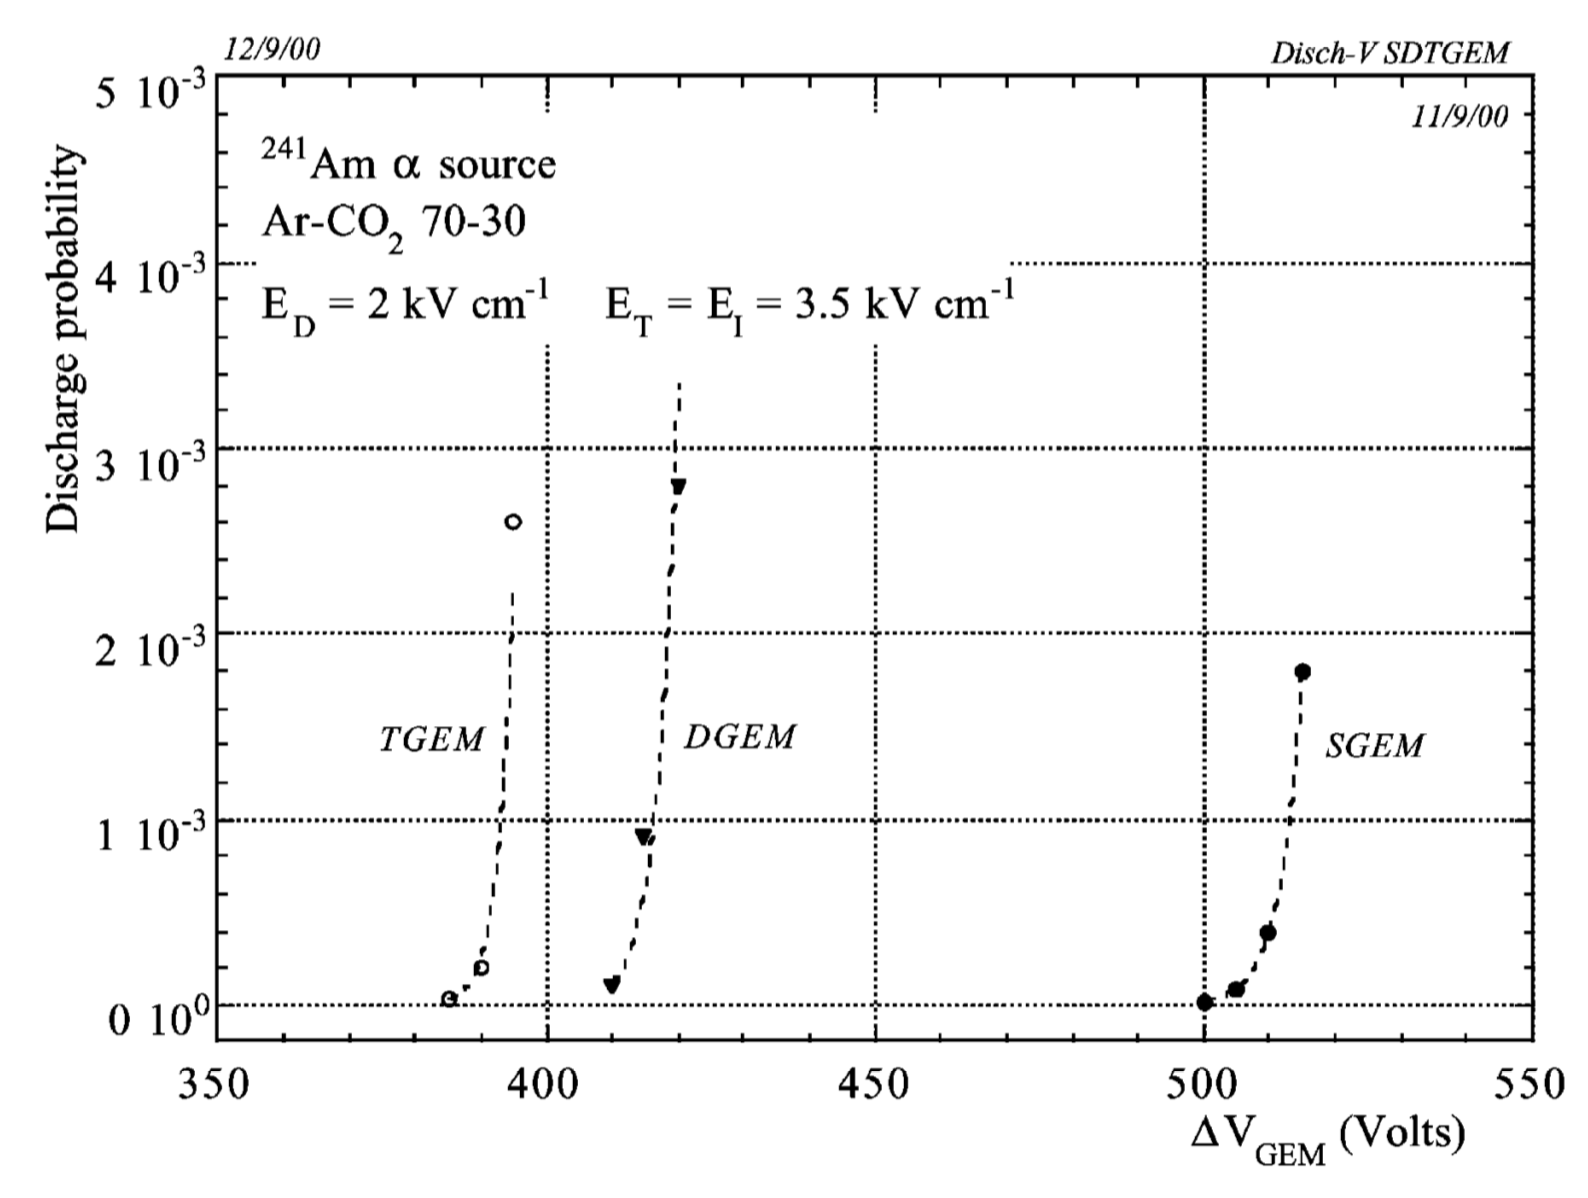
\includegraphics[width=0.45\textwidth]{figures/GEM/Comp_threeGEMS_DischargeProbability.png}
    \caption{Left: Comparison of total effective gain on anode as a function of applied voltage for single, double and triple GEM detectors. Right: Comparison of discharge probability as a function of applied voltage on anode for single, double and triple GEM detectors~\cite{Bachmann2002}.}
    \label{fig:tripleGEM_discharge_gain}
\end{figure}
% section design_and_working_principle_of_gem (end)


\section{GEM For CMS Phase-II Upgrade} % (fold)
\label{sec:gem_for_cms}
As discussed in Sec.~\ref{sub:the_muon_system},  the CMS collaboration finalizes to install the GEM detector in region $1.6 < |\eta| < 2.2$ to support the CSC muon sub-system and improve the triggering and tracking capability of the muons in the forward region~\cite{Colaleo:2021453}. 
The upgrade target for the proposed upgrade is:
    \begin{itemize}
        \item Re-establish the redundancy in the difficult region beyond $\eta = 1.6 $
        \item Improve tracking performance in the high rate environment
        \item The combined operation of CSC and GEM detectors allows a measurement of the bending angle at the trigger level, thus strongly reducing the rate of mis-measured muons driving the triggers rate.
    \end{itemize}
% \subsection{GE11 Details}
The installation of GEM detectors is proposed during the Long Shut-down 2(2019-2020).
The project is named GE1/1, where ``G'' stands for GEM, ``E'' stands for End-cap, the first ``1'' corresponds to the first muon station and the second ``1'' the first ring of the station.
Also, the GEM detector which is going to install in the CMS is named as a GE11 detector.
The detectors will be inserted in front of the ME1/1 station in the slots originally foreseen for RPC detectors as shown in Fig.~\ref{fig:GE11pos}. 
\begin{figure}[!htbp]
    \centering
    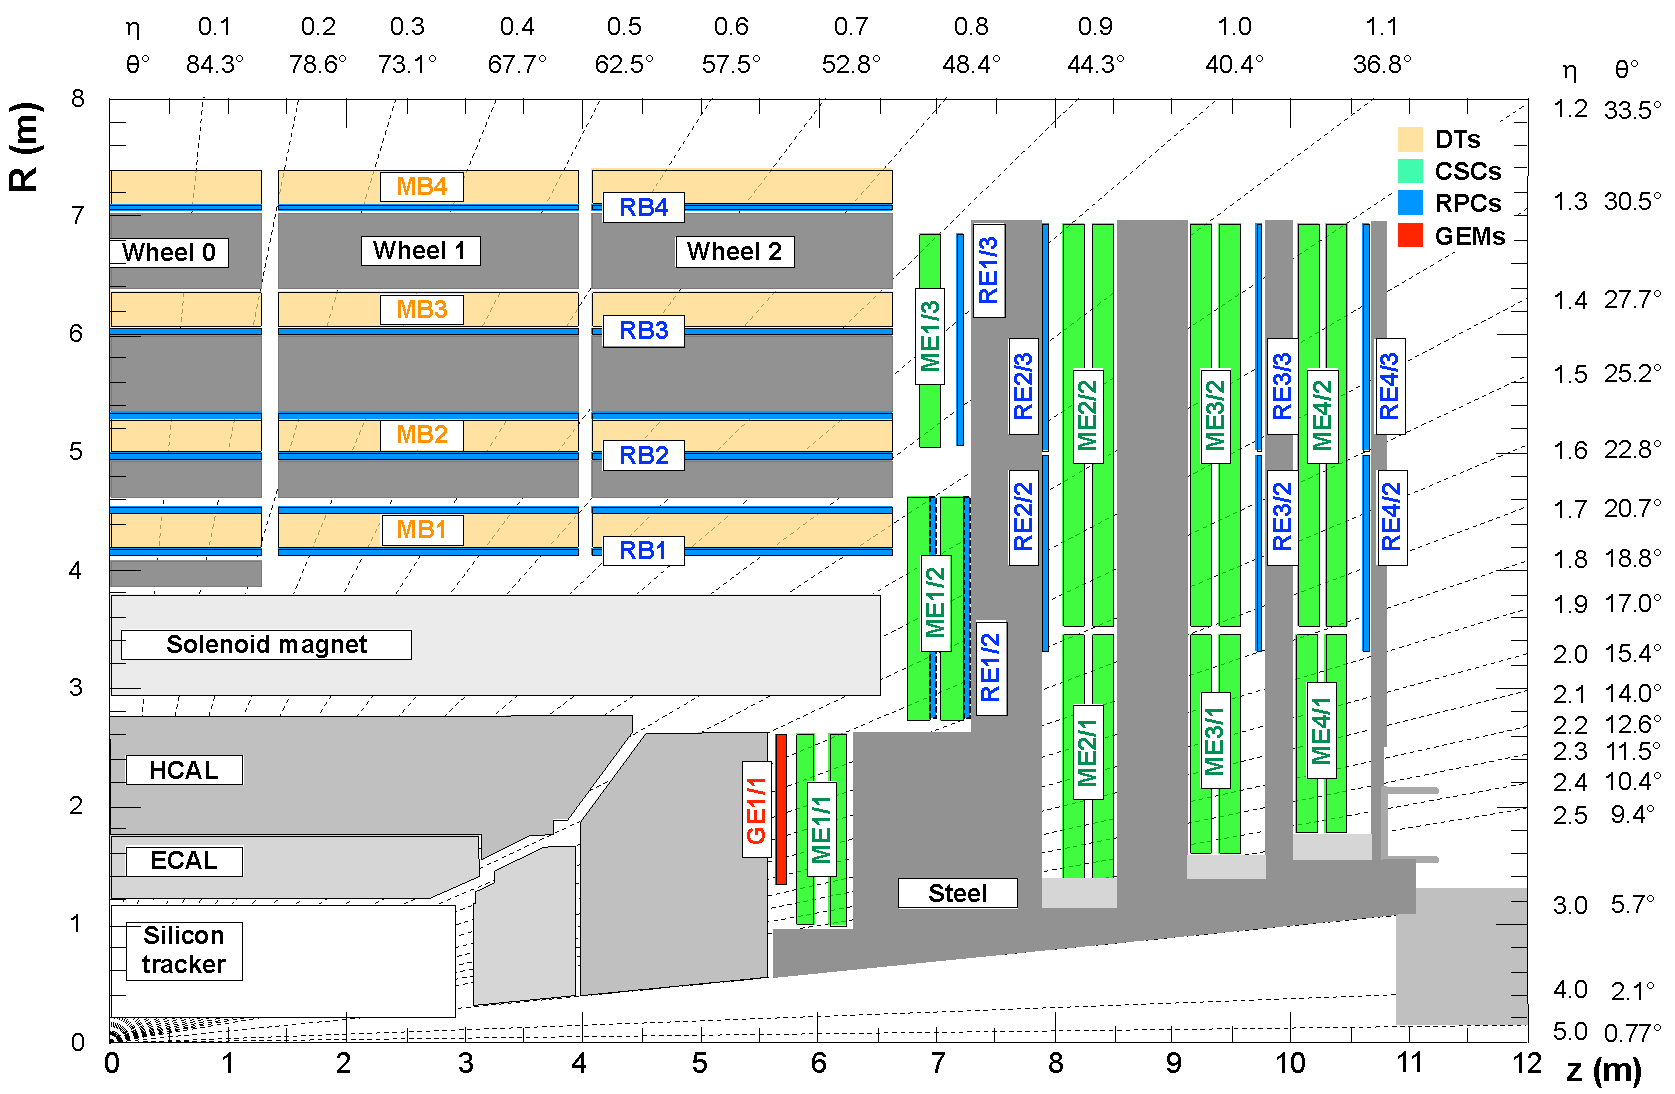
\includegraphics[width=0.95\textwidth]{figures/GEM/cms_upg_o_g_b_ni_ge1_r_140227.pdf}
    \caption{A cross-sectional view of CMS quadrant showing the location of GEM detectors in red.}
    \label{fig:GE11pos}
\end{figure}

\subsection{CMS GE11 Detector Details} % (fold)
\label{sub:ge11_detector_details}
A GE11 detector is trapezoidal in shape with an active area of $990\times (220-445)mm^2$.
This size was imposed by the geometry of the vacant high-$\eta$ area in CMS muon endcap.
GE11 chamber hosts a Triple-GEM detector with a $3/1/2/1~mm$ (drift/transfer 1/transfer 2/induction) electrode gap configuration, as shown in Fig. \ref{fig:tripple-gem}.
\begin{figure}[!htbp]
    \begin{center}
        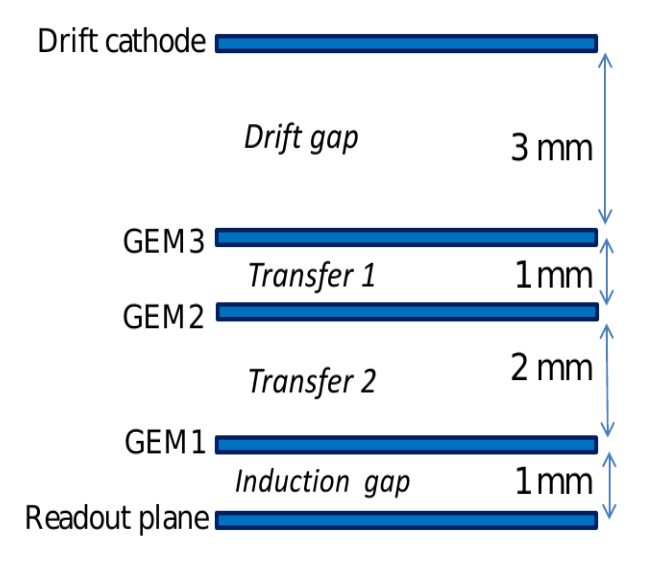
\includegraphics[width=0.45\textwidth]{figures/GEM/tripple-gem.png}
        \caption{Cross-section of the proposed triple-GEM showing the dimensions of the different gaps}
        \label{fig:tripple-gem}
    \end{center}
\end{figure} 
The GEM foil ($50~\mu m$ thick Kapton foil with $5\mu m$ copper on both sides) consists of a thin Kapton foil, metal-clad on both sides.
The detector readout board is divided into eight $\eta$-partitions with 384 strips each oriented radially along the long side of the detector with a pitch varying from $0.6mm$ (short side) to $1.2mm$ (long side).
Each partition is subdivided along the $\phi$-coordinate into three readout sectors with 128 strips or channels each. The $\eta$ partition and $\phi$ portions are shown in Fig.~\ref{fig:gemTrapezoidal}.
\begin{figure}[!htbp]
    \begin{center}
        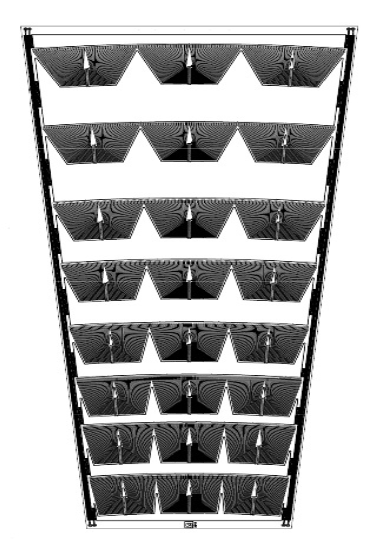
\includegraphics[angle=-90,width=0.75\textwidth]{figures/GEM/gemTrapezoidal.png}
        \caption{Drawing of a large trapezoidal CMS GEM chamber showing $8-\eta$ and $3-\phi$ par partitions.}
        \label{fig:gemTrapezoidal}
    \end{center}
\end{figure} 
To improve tracking capabilities, two GEM chambers will be mounted face-to-face to form a double layer called ``\textit{Super-Chamber}".
Thus each Super-Chamber will provide two impact points for each muon track.
The full layer by layer design of the GEM chamber is shown in Fig.~\ref{fig:ge11}. 
The main parts in a GEM detector are GEM foil, drift plane, readout board, shielding, high voltage divider, etc.
\begin{figure}[!htbp]
    \begin{center}
        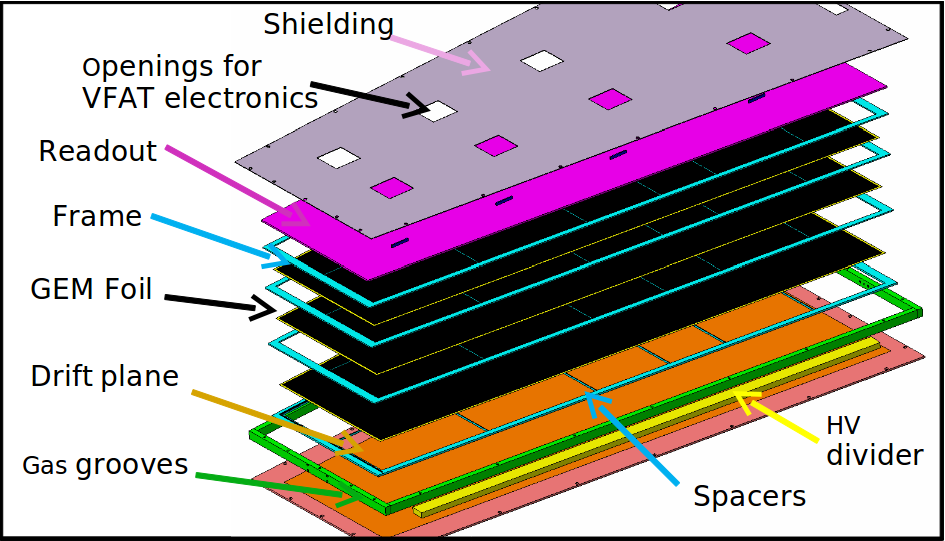
\includegraphics[width=0.95\textwidth]{figures/GEM/ge11cad.png}
        \caption{Layer by layer view of GEM detector}
        \label{fig:ge11}
    \end{center}
\end{figure} 
\todo[inline]{Add a para on fig~\ref{fig:ge11}}
\todo[inline]{Add a para on GE11 fabrication}
% \begin{figure}[!htbp]
% \centering
% 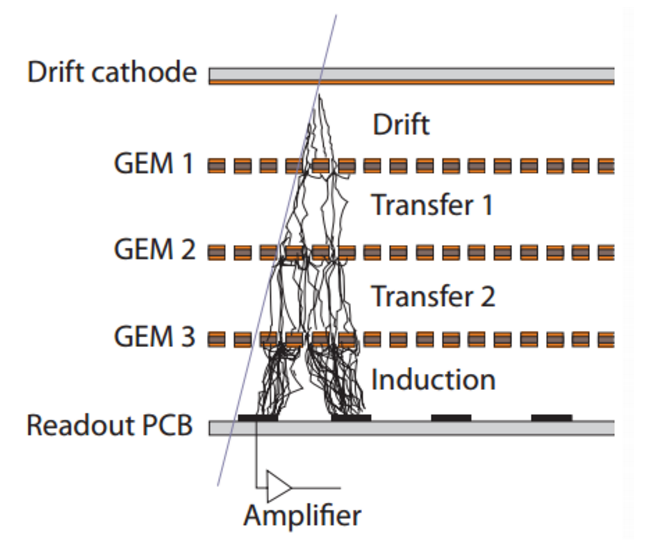
\includegraphics[width=2.0in]{figures/GEM/GEMCascade.png}
% \caption{Generic triple-GEM chamber, showing drift, transfer, and signal induction gap regions within the detector.}
% \label{GEM:cascade}
% \end{figure}

\subsection{GE11 Test Beam}
The GE11 detector was tested using 150 GeV muon and pion beams at CERN SPS test beam during October-December 2014. The goal of the test beam was to measure the gain, noise, efficiency, space \& time resolution, and cluster size. The detector that was tested are GE11\_IV\_CERN\_0001 and GE11\_IV\_CERN\_0002 (detectors naming convention and its details are mentioned in appendix~\ref{cha:ge11_detector_generations}). Also there was two test beam held in October-December 2014. These two held in H2 and H4 test beam area of CERN SPS. H2 test beam held from $6^{th}$ October 2014 to $27^{th}$ October 2014. And, H4 test beam was held from 26 November to 14 December 2014. The main goal of the H2 test beam was to test the two detectors mentioned above with $Ar:CO_2$ gas while in H4 test beam the same was test with gas mixture $Ar:CO_2:CF_4$. Initially, the plan was to scan the each sector of the GEM detectors while due to time and other constraints we were just able to scan sector $(i\eta, i\phi)=\{(5,2)\}$ but while H4 we scanned $(i\eta,i\phi)=\{(1,2),(5,2),(8,2)\}$.  

Further mainly based on the electronics used we divided all the data taken in different run numbers. Out of them there are 4 golden run (i.e. of good quality that we analyzed for further studies). It is listed in table~\ref{tab:gemTBgoldenruns}.

\begin{table}
\begin{tabular}[!htbp]{l l}
\hline
\textbf{Run Name}   &   \textbf{Details}\\
\hline
2014H2C     & Run range: 306-407    \\
            & Threshold for each VFAT strip = 15 VFAT units\footnote{1 VFAT unit = 0.08 fC} = 1.2fC\\
            & Runs in async mode \\
            & sector scanned $(i\eta, i\phi)=(5,2)$\\
            & gas used: $Ar:CO_{2}$=(70:30)\\
\hline
2014H4A     & Run range: 1592-1646 \\
            & Threshold for each VFAT strip = 15 VFAT units = 1.2fC\\
            & Runs in async mode \\
            & sector scanned $(i\eta, i\phi)=(5,2)$\\
            & gas used: $Ar:CO_{2}:CF_4$=(40:15:45)\\
\hline
2014H4C     & Run range: 1868-1906 \\
            & Threshold for each VFAT strip = 15 VFAT units = 1.2fC\\
            & Runs in async mode \\
            & sector scanned $(i\eta, i\phi)=(8,2)$\\
            & gas used: $Ar:CO_{2}:CF_4$=(40:15:45)\\
\hline
2014H4D     & Run range: 2065-2123 \\
            & Threshold for each VFAT strip = 15 VFAT units = 1.2fC\\
            & Runs in async mode \\
            & sector scanned $(i\eta, i\phi)=(1,2)$\\             
            & gas used: $Ar:CO_{2}:CF_4$=(40:15:45)\\
\hline
\end{tabular}
\caption{List of golden runs that are analyzed to extract the GEM properties.}
\label{tab:gemTBgoldenruns}
\end{table}



A gas mixture used for the test beam campaign is $Ar:CO_{2}$ (70:30) and $Ar:CO_{2}:CF_{4}$ (40:15:45).
% subsection ge11_detector_details (end)


\subsection{Experimental Set-up}
% A simple schematic diagram of the experimental setup is shown in Fig.~\ref{fig:tbsetup}.
The experimental set-up consists of three plastic organic scintillators, three trackers and a GE1/1 prototype, being flushed with an Ar/CO$_{2}$ (70:30) gas mixture. The trackers are triple-GEM detectors with a $10~cm\times10~cm$ active area. Each tracker has 256 strips in both horizontal (y-coordinate) and vertical (x-coordinate) directions transverse to the beam having the pitch of $0.4~mm$. Trackers constitute a muon tracking telescope which is used to reconstruct the beam trajectories and reduce background events. Figure~\ref{fig:tbs} shows the experimental set-up used to perform test beam studies.
% \begin{figure}[!htbp]
%     \begin{center}
%         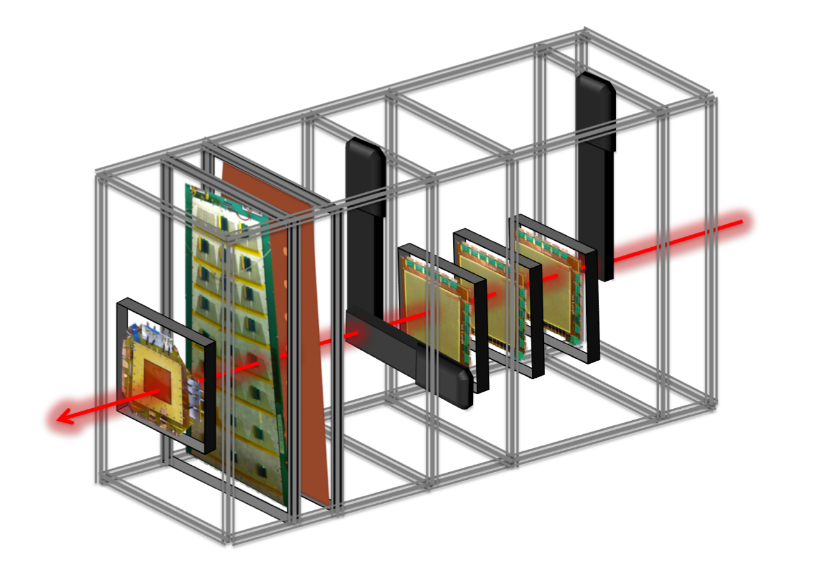
\includegraphics[width=0.95\textwidth]{figures/GEM/tbsetup.png}
%         \caption{Schematic view of the test beam set-up with the three square GEM hodoscope and the trapezoidal CMS GEM chambers}
%         \label{fig:tbsetup}
%     \end{center}
% \end{figure} 
\begin{figure}[!htbp]
\centering
% 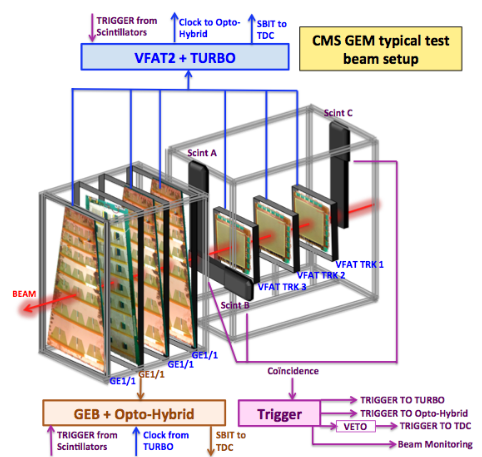
\includegraphics[width=0.95\textwidth]{figures/GEM/tb_exptsetup.png}
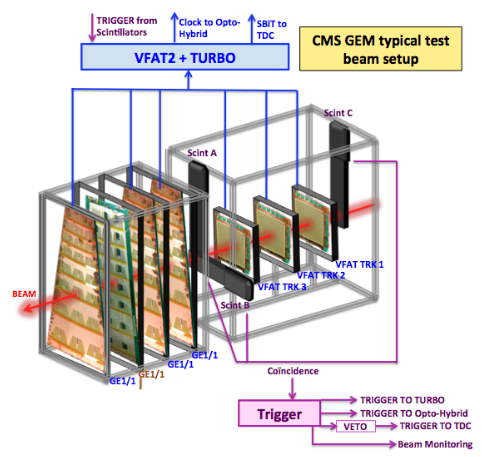
\includegraphics[width=0.95\textwidth]{figures/GEM/tb_exptsetup_copy.png}
\caption{Schematic view of the test beam set-up with the three square GEM hodoscope and the trapezoidal CMS GEM chambers. Also, it shows the trigger generation and timing DAQ systems}\label{fig:daq}
\end{figure}
On Detector electronics connect the inputs of the front-end ASIC (VFAT2) to the GEM readout board.
The VFAT2 is connected to the hybrids which are plugged into the connectors on the readout board.
%The trigger is generated using the coincidence of three photo-multiplier tubes with mounted scintillators. 
The tracking telescope is equipped with the digital chips VFAT2~\cite{Aspell:2008zz}, which provides a binary output with a variable latency for the position information and a fixed latency output, called SBIT, for the timing information.
The analog pulses from the three scintillators, named S1, S2 and S3, are converted into digital gates after discriminator units and put in coincidence (to generate event trigger) before being sent to the other DAQ systems (Figure.~\ref{fig:daq}).
\begin{figure}[!htbp]
\centering
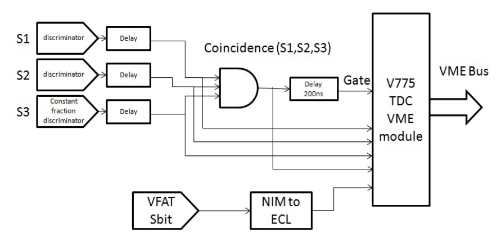
\includegraphics[width=0.95\textwidth]{figures/GEM/daq.png}
\caption{Perspective view of the typical experimental set-up for performance measurement in the test beam. The tracking telescope is made of three triple-GEM detectors with two orthogonal directions readout. The trigger system is ensured thanks to three scintillators connected in coincidence. The GE1/1 detectors under test are mounted onto a movable support to align various readout sectors with the beam line.}\label{fig:tbs}
\end{figure}
The active area of the GE1/1 detector is covered with readout strips located in the GEM Electronic Board. 
The readout strips are taken out in 24 readout sectors (in ($\eta$,$\phi$) phase space).
The data of each sector is collected by a VFAT2 font-end chip. 
% An upgraded version of this chip is currently under development (\textbf{VFAT3}). 
% Each VFAT2 builds a data packet that is sent through an e-link to an on-detector component called opto-hybrid (OH). 
% The OH serializes the data and sends them to the off detector components via an optical link. 
% The OH also receives the triggering information sent by the off-detector components of the system. 
% The off-detector electronics, based in a $\mu$TCA crate technology, are the interface with CMS central systems: DAQ, trigger, etc. 
% The OH sends the data to an AMC (Advanced Mezzanine Card) type card CTP7. The CTP7 sends the data to an AMC13 card through the mTCA back-plane. 
% The AMC13 card communicates directly with the central CMS DAQ system.
%The trigger is generated using the coincidence of three photo-multiplier tubes with mounted scintillators. 

The GE1/1 prototypes are installed on a movable table to scan different detector sectors. At a time only one ($\eta$,$\phi$) sector of GEM detector is irradiated with the beam.
% The high voltage powering was realized using a ceramic high voltage divider. 
The CMS test chamber was placed, close to the tracking hodoscope, on a vertically movable support to allow scanning.  The scanned sectors of the GE11 detector are shown in Fig.~\ref{GE11}
%, with a tracker pitch of $0.4~mm$
\begin{figure}[!htbp]
\centering
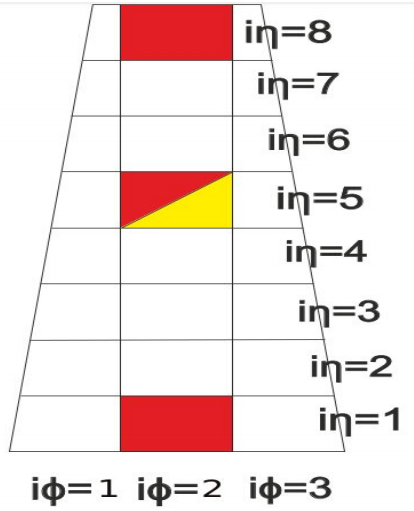
\includegraphics[scale=0.5,angle=90]{figures/GEM/GE11.png}
\caption{Different $(i\eta,i\phi)$ sectors of full-size GE1/1 detector prototype. The red and yellow colour shows which sector of GE1/1's are exposed to the beam. Red sectors are taken with gas $Ar/CO_2/CF_4~(45/15/40)$ while the yellow sector is taken with gas $Ar/CO_2~(70/30)$.}
\label{GE11}
% THis is for test beam
\end{figure}
\subsection{Results} % (fold)
\label{sub:results}

\subsubsection{Basic Results} % (fold)
\label{ssub:basic_results}
Fig.~\ref{BeamProfile} shows a beam profile of the muon beam as reconstructed with three trackers. The beam, shown in red, is centered around (50,50) for the three trackers.
\begin{figure}[!htbp]
\centering
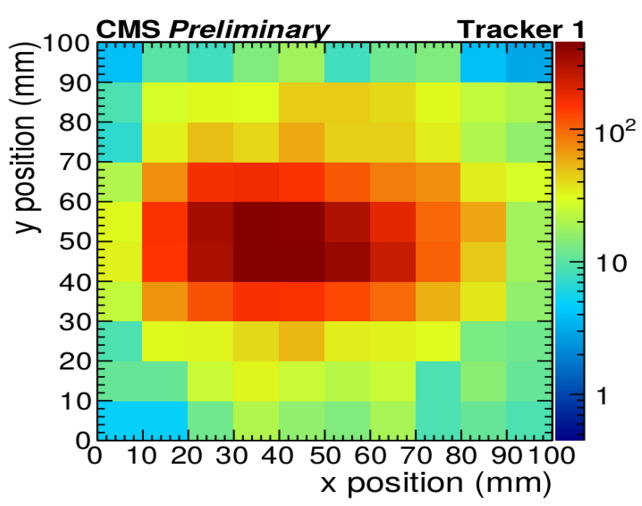
\includegraphics[width=0.35\textwidth]{figures/GEM/Selection_027.png}%
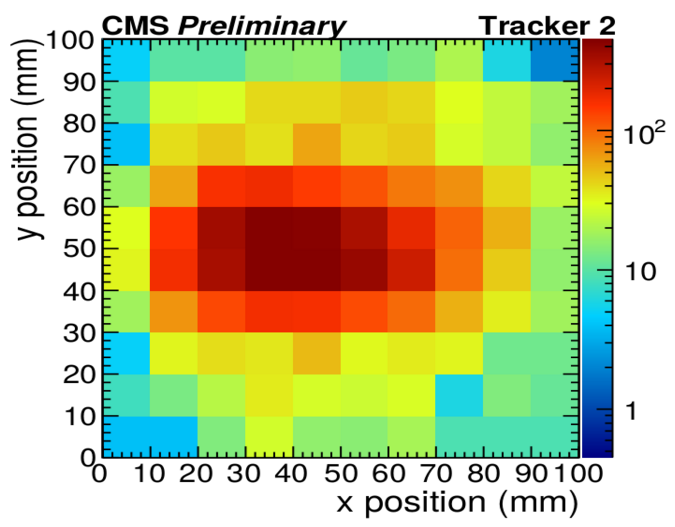
\includegraphics[width=0.35\textwidth]{figures/GEM/Selection_028.png}%
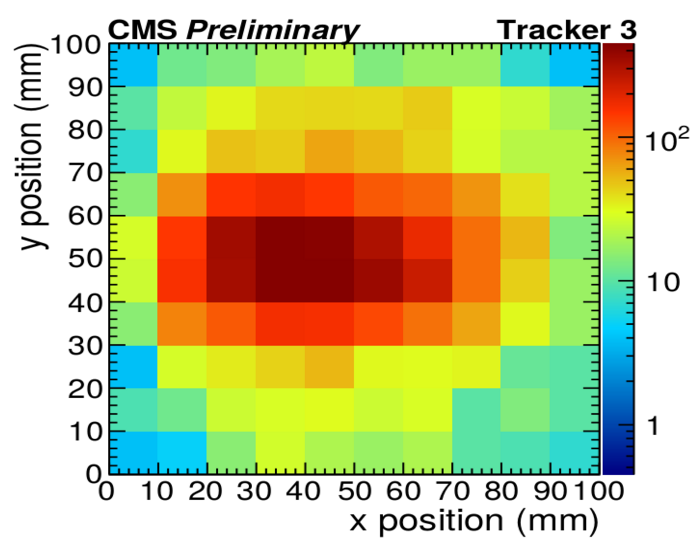
\includegraphics[width=0.35\textwidth]{figures/GEM/Selection_029.png}
% where an .eps filename suffix will be assumed under latex, 
% and a .pdf suffix will be assumed for pdflatex; or what has been declared
% via \DeclareGraphicsExtensions.
\caption{2D- beam profile plot for the first, second and third tracker. The X and Y axis correspond to the distance (in mm) measured from the central position of the trackers in X and Y direction, respectively. The different colors in the color palette correspond to the number of hits registered in the detector at a particular (x,y) position.}\label{BeamProfile}
\end{figure}
And Fig. \ref{HitPosXaxis} represents the tracker and GE1/1 hit positions along x and y-direction.
\begin{figure}[!htbp]
\centering
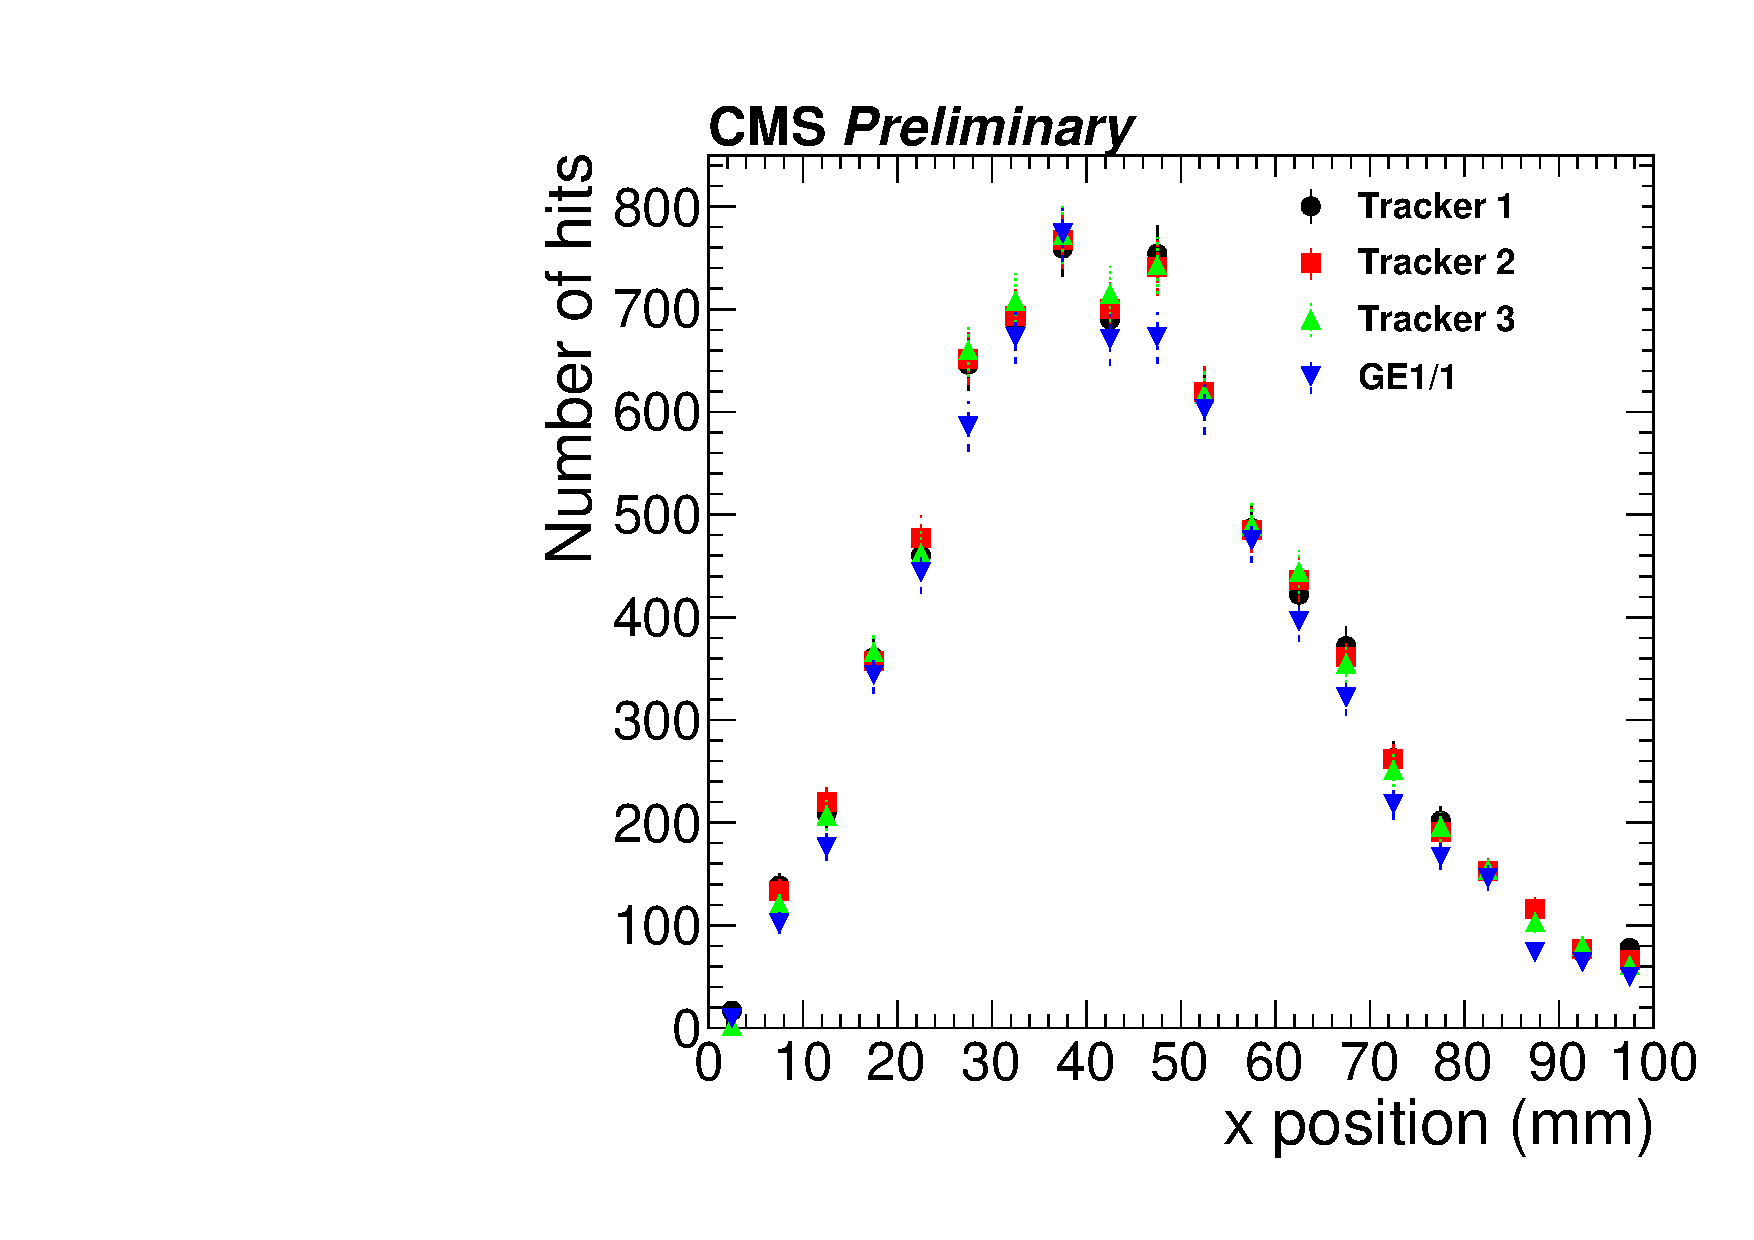
\includegraphics[width=0.45\textwidth]{figures/GEM/Tracker_Hit_position_Run1644_x.pdf}%
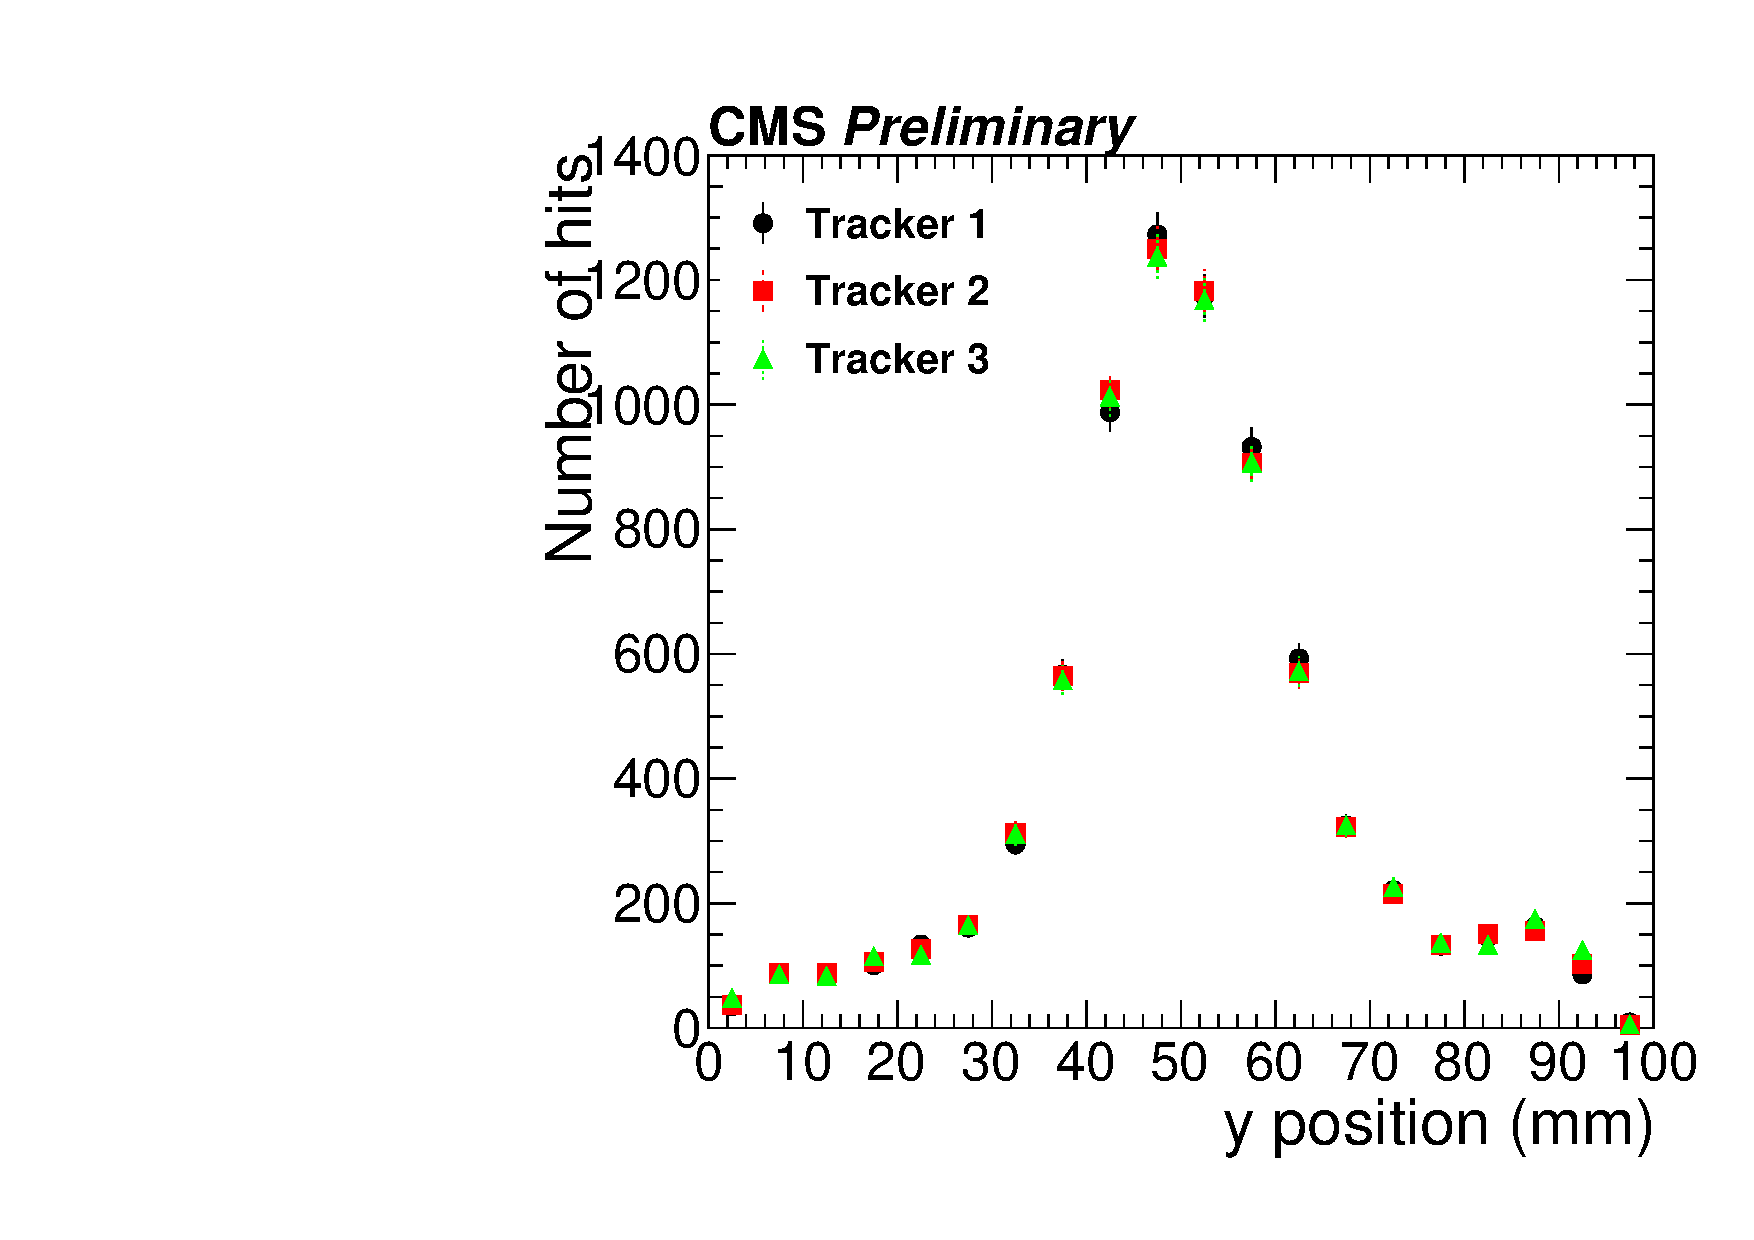
\includegraphics[width=0.45\textwidth]{figures/GEM/Tracker_Hit_position_Run1644_y.pdf}
\caption{Tracker hit distribution along x and y axis and GE1/1 hit distribution along y. This is plotted from one of run taken during test-beam.}
\label{HitPosXaxis}
\end{figure}

% subsubsection basic_results (end)ub
\subsubsection{Alignment Studies}

In order to reconstruct an ionizing particle trajectory, it is needed to detect the positions of the incoming particles within the space. 
The technique used for this purpose consists of the interposition along the trajectory of several detector planes where the particles pass through; from the interpolation of all these points can be reconstructed the trajectories followed by the particles.
In these environments one of the most important merit figures of the detectors is the spatial resolution, that is the capability to reconstruct the crossing point of the particle.
% Basically, the evaluation of the spatial resolution of a particle detector consists on the irradiation of the detector under test with particles beam at high energy and on the measurement of the differences between the measured impact points with the real ones.
% It is clear that it is necessary to know the real impact points of the incoming particles, a solution of this problem is to use a known tracking system (usually called telescope) with which it is possible to measure this positions.
\begin{figure}[htbp]
    \centering
    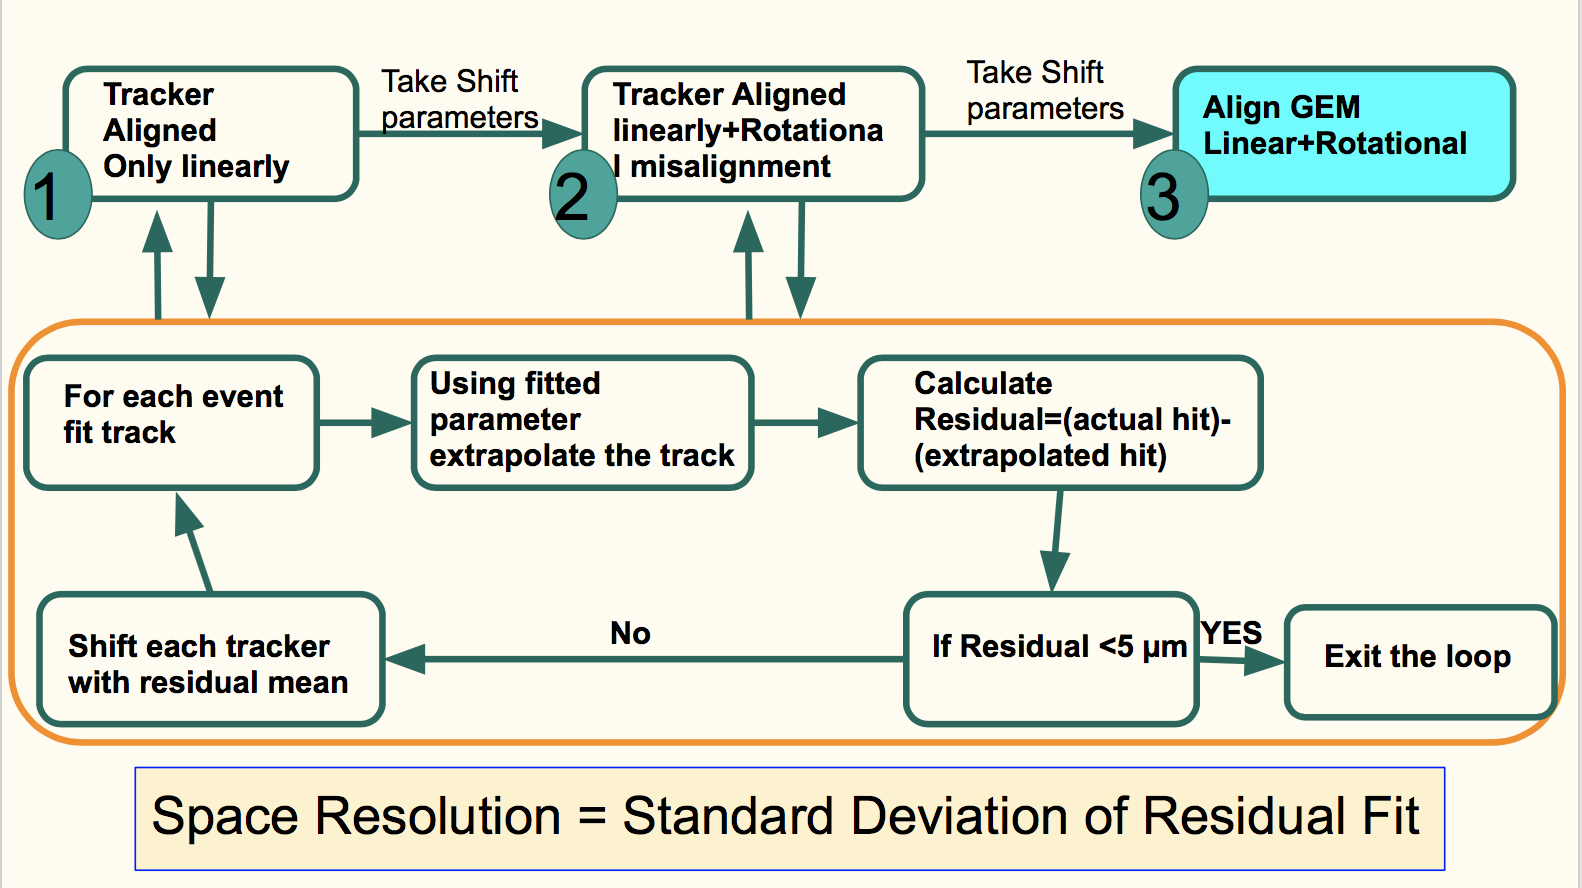
\includegraphics[width=0.95\textwidth]{figures/GEM/GEM_Alignment_FlowChart.png}
    \caption{caption}
    \label{fig:label}
\end{figure}
% Offline, track-based alignment is one of the fundamental reconstruction tasks which needs to be accomplished in order to fully exploit physics potential of high-resolution position-sensitive particle detectors.
% It is needed to assure high-quality reconstruction of charged particles, interaction vertices, resonance masses, etc.
% The large and accurate vertex detectors of present and future experiments have a potential measurement precision of a few $\mu$ m.
% If this is not satisfied particle trajectories are reconstructed with compromised resolution, often with reduced efficiency and subject to systematic biases.
% In addition to the initial optical survey and corrections for electronics and mechanical effects the use of tracks in a special software alignment is essential.
% A number of different software-based methods are in use, ranging from simple residual-based procedures to complex fitting systems with many thousands of parameters.

Alignment/calibration requires to understand the detector (functional relationship) and to optimize various detector  parameters.
The goal is to reduce the $\chi^{2}$ of the track fits, in order to improve track and vertex recognition, and to increase the precision of reconstructed tracks and vertices, eliminating or reducing bias in detector data.
Current detector alignment studies are performed using the data collected during 2014 the beam test of GEM detectors. 
% The test-stand set-up used to take data consists of three small FIXME dims GEM trackers placed parallel to beam direction followed by CMS GEM detectors. 
%%%FIXME describe the system
%% Run1897_Muons_10k_MSPL4_Async_HVScan_770pt2_788pt8_0pt0_758pt4_769pt9_T15_Lat17
% Current studies are performed for a muon run taken during test beam with 10k events.
% Figure.~\ref{fig:t1bp}, Figure.~\ref{fig:t2bp} and Figure.\ref{fig:t3bp} show the beam profile recorded on Tracker 1, Tracker 2 and Tracker 3 respectively. 
% Red box at the center indicates the maximum hit positions on X and Y readouts.
% \begin{figure}[!htbp]
%     \centering
%     \begin{subfigure}[b]{0.46\textwidth}
%         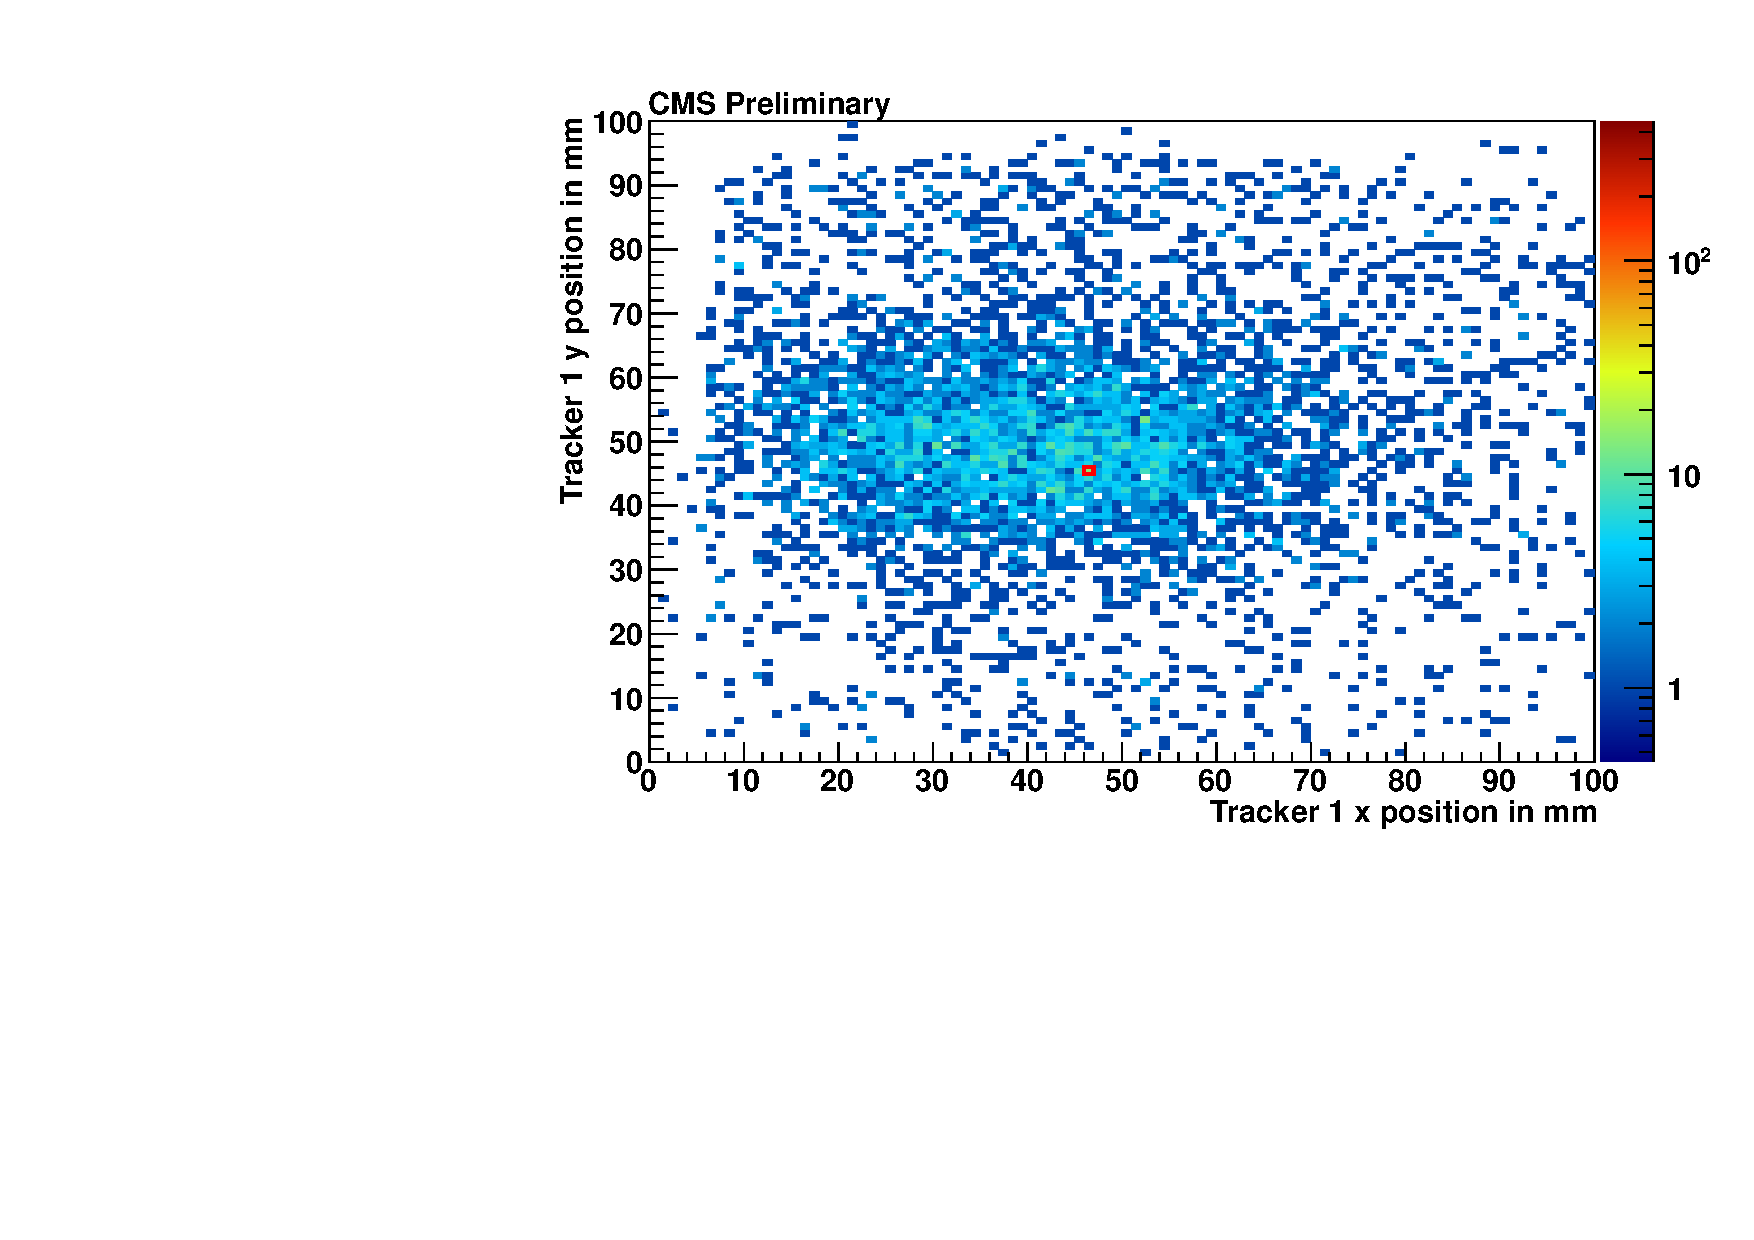
\includegraphics[scale=0.35]{figures/GEM/profile_plots_for_Tracker1_Run1897.pdf}
%         \caption{ }
%         \label{fig:t1bp}
%     \end{subfigure}
%     \begin{subfigure}[b]{0.46\textwidth}
%         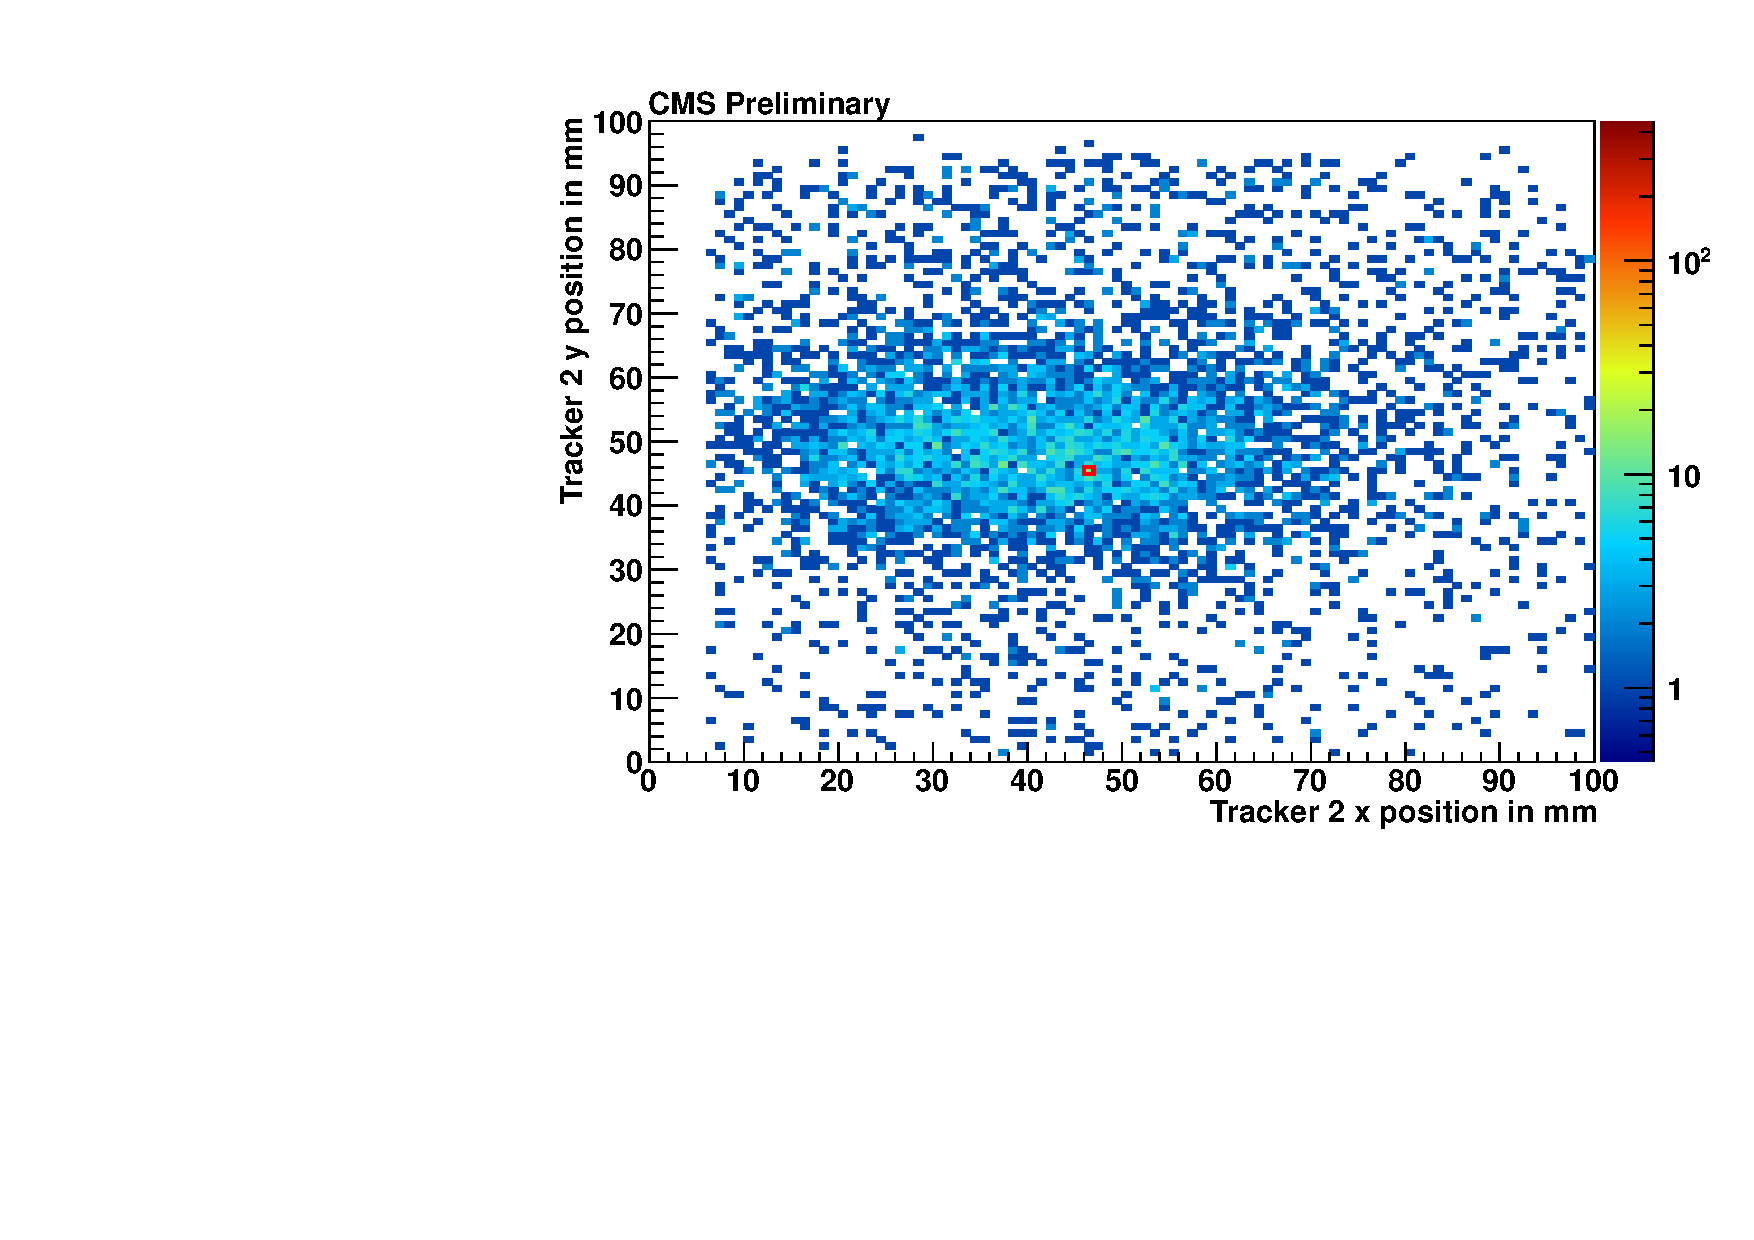
\includegraphics[scale=0.35]{figures/GEM/profile_plots_for_Tracker2_Run1897.pdf}
%         \caption{ }
%         \label{fig:t2bp}
%     \end{subfigure}
%     \begin{subfigure}[b]{0.46\textwidth}
%         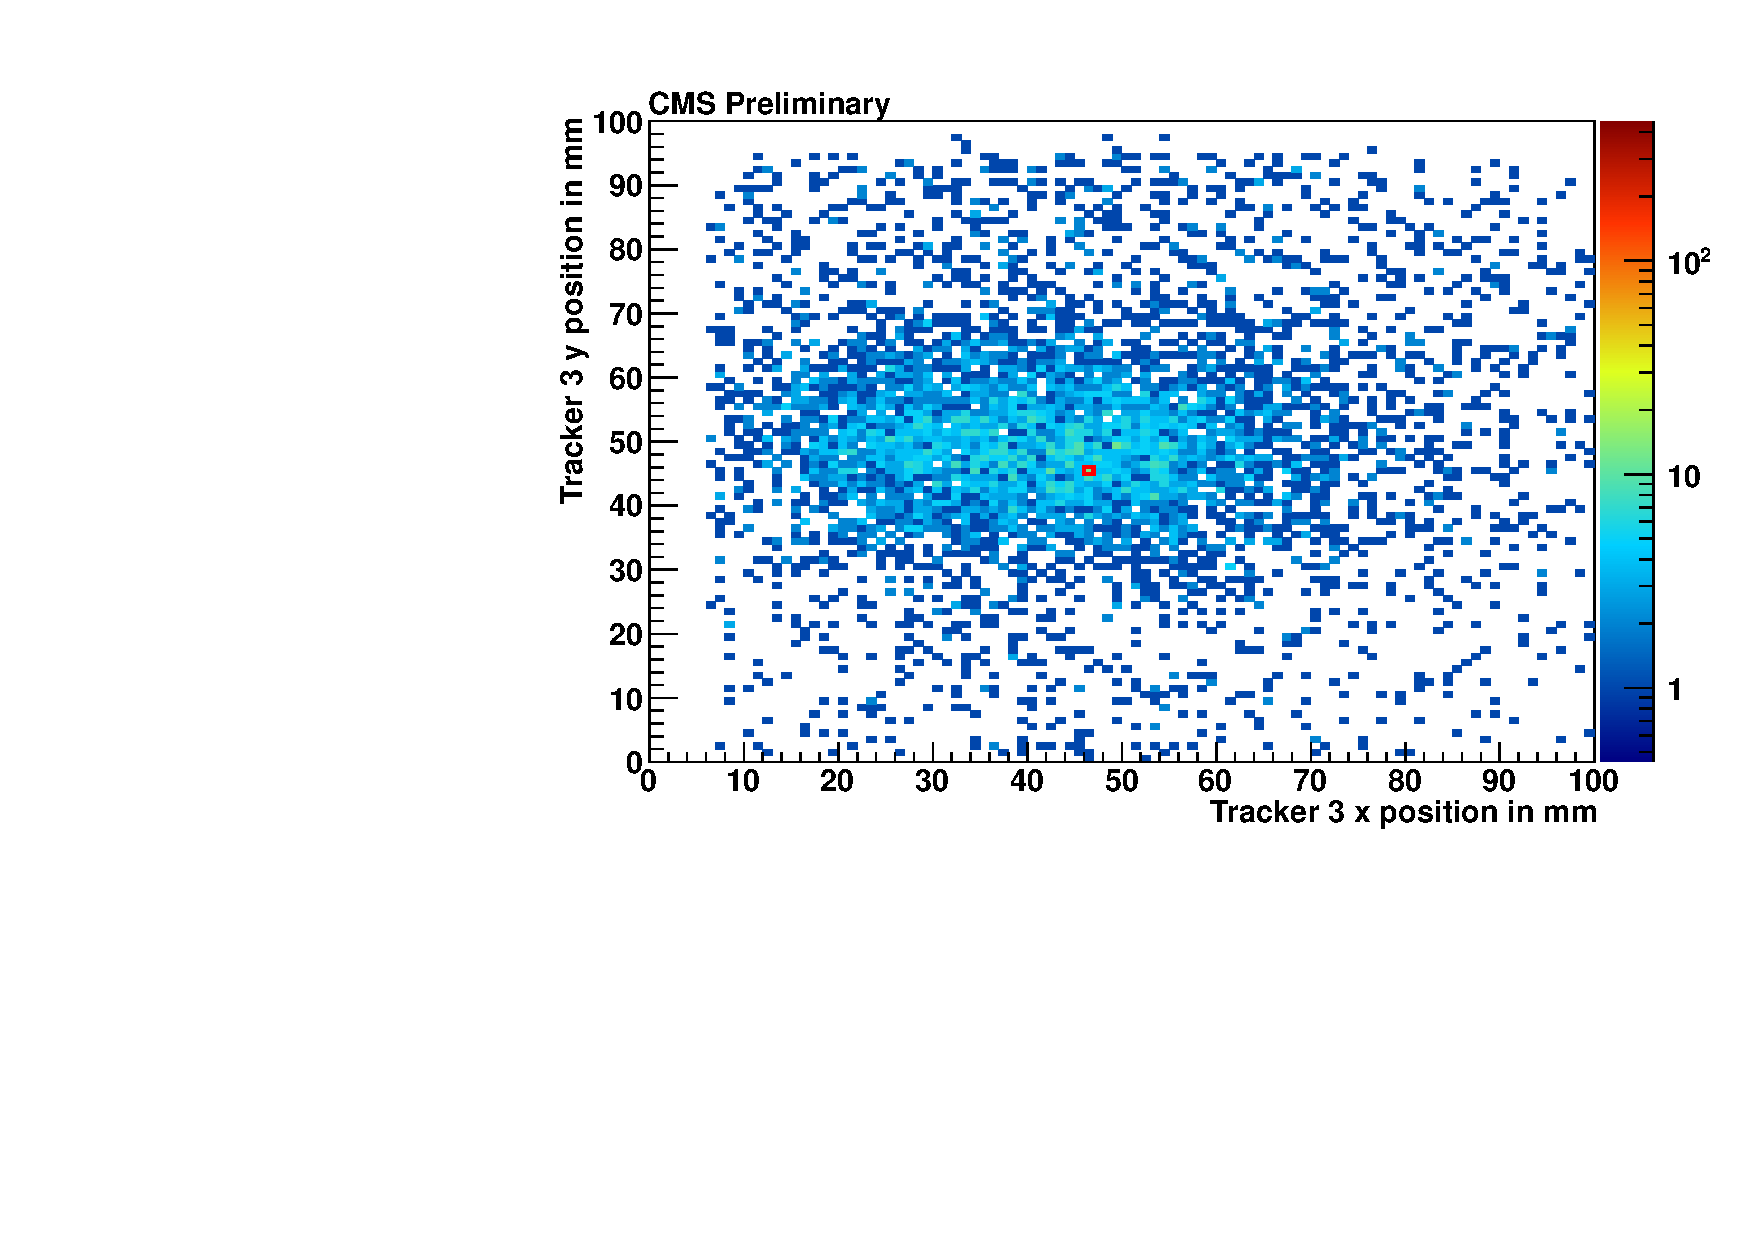
\includegraphics[scale=0.35]{figures/GEM/profile_plots_for_Tracker3_Run1897.pdf}
%         \caption{ }
%         \label{fig:t3bp}
%     \end{subfigure}
%    \caption{(a) 10 cm $\times$ 10 cm GEM foil encapsulated in a frame and (b) Cross-sectional view of the foil showing the double cone structure of the engraved holes. } \label{fig:Foil_and_Cone}
% \end{figure}
% Fig.~\ref{fig:t1hit},~\ref{fig:t2hit}, and~\ref{fig:t3hit} show the hit positions for three trackers in X and Y direction. Clearly the maximum hit positions are not located at the centre of the trackers (before software alignment).
% \begin{figure}[!htbp]
% \centering
% 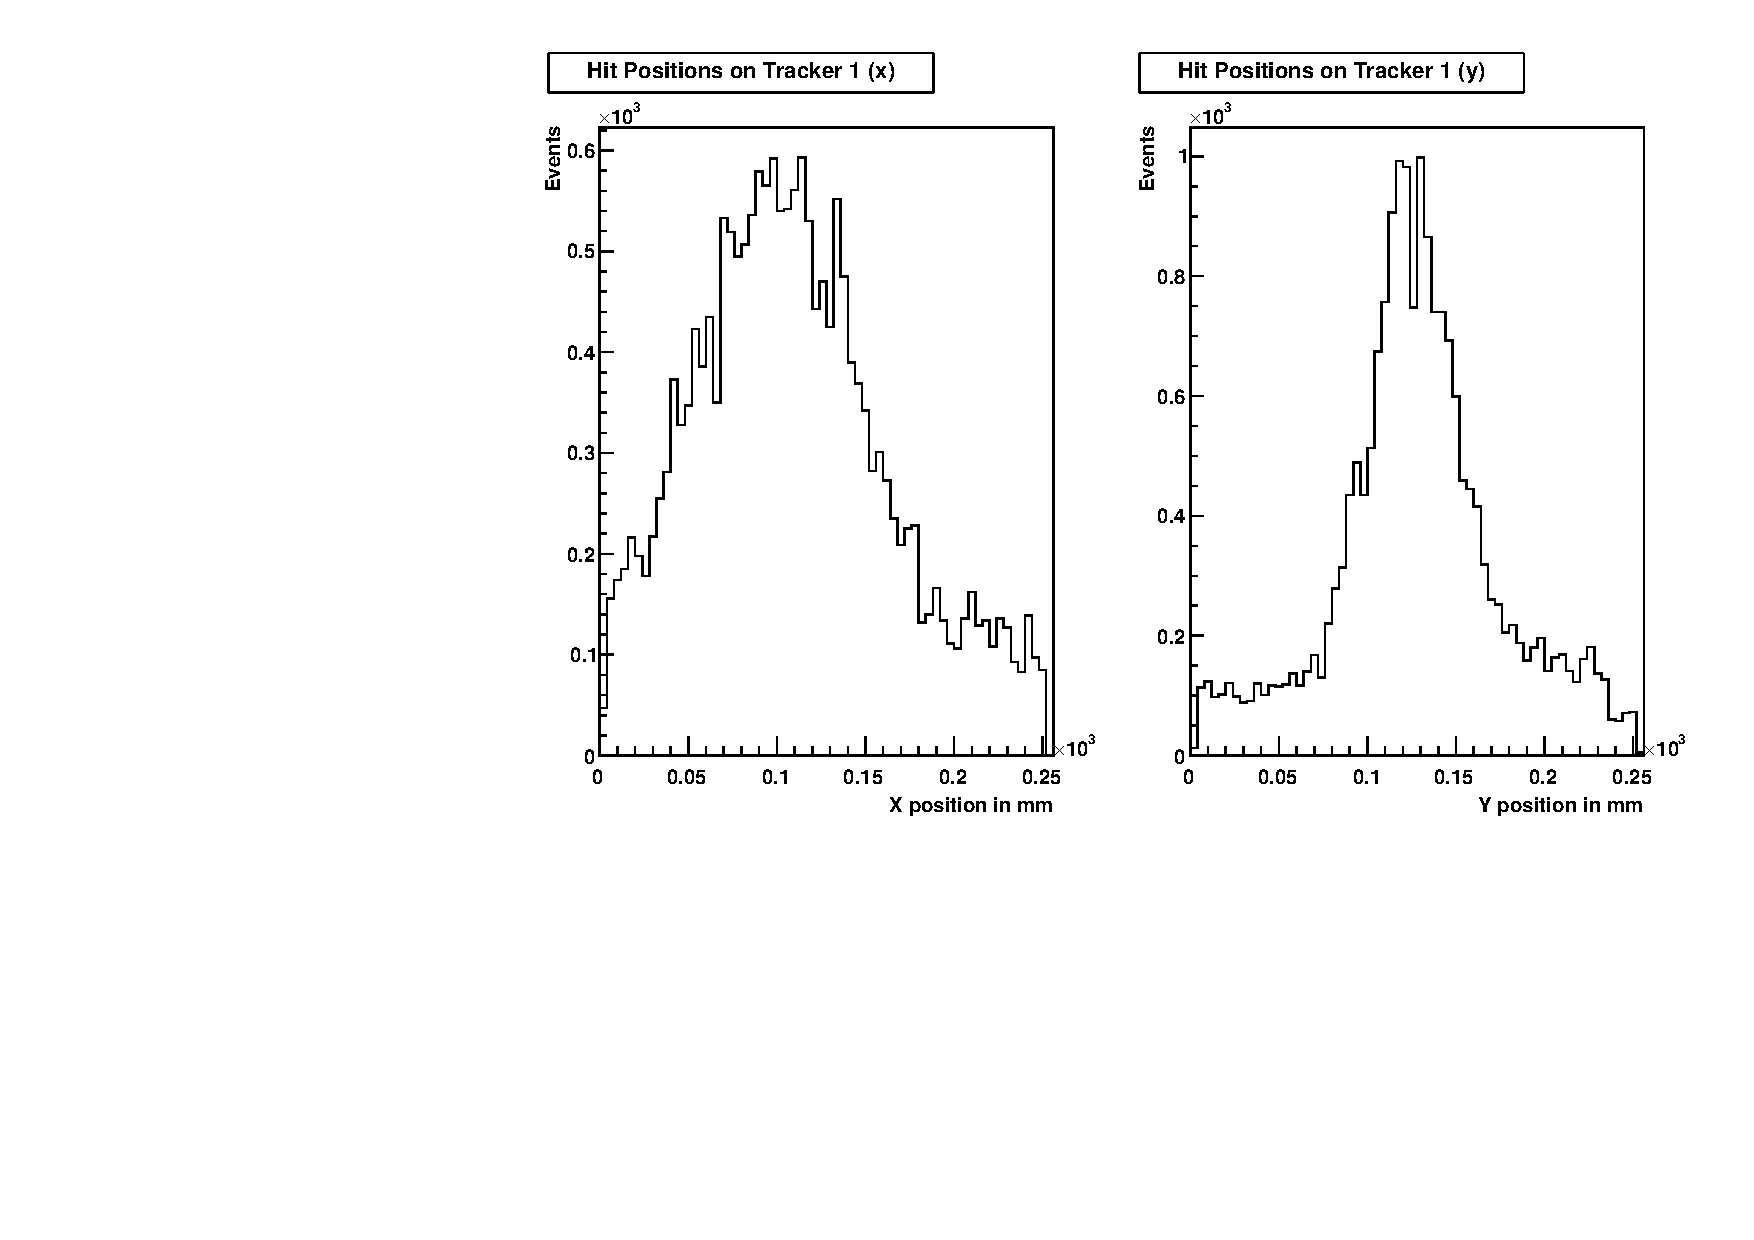
\includegraphics[width=5.1in]{figures/GEM/Tracker1_Hit_position_Run1897.pdf}
% \caption{Tracker 1 hit positions in X direction(left) and Y direction(right)}\label{fig:t1hit}
% \end{figure}
% \begin{figure}[!htbp]
% \centering
% 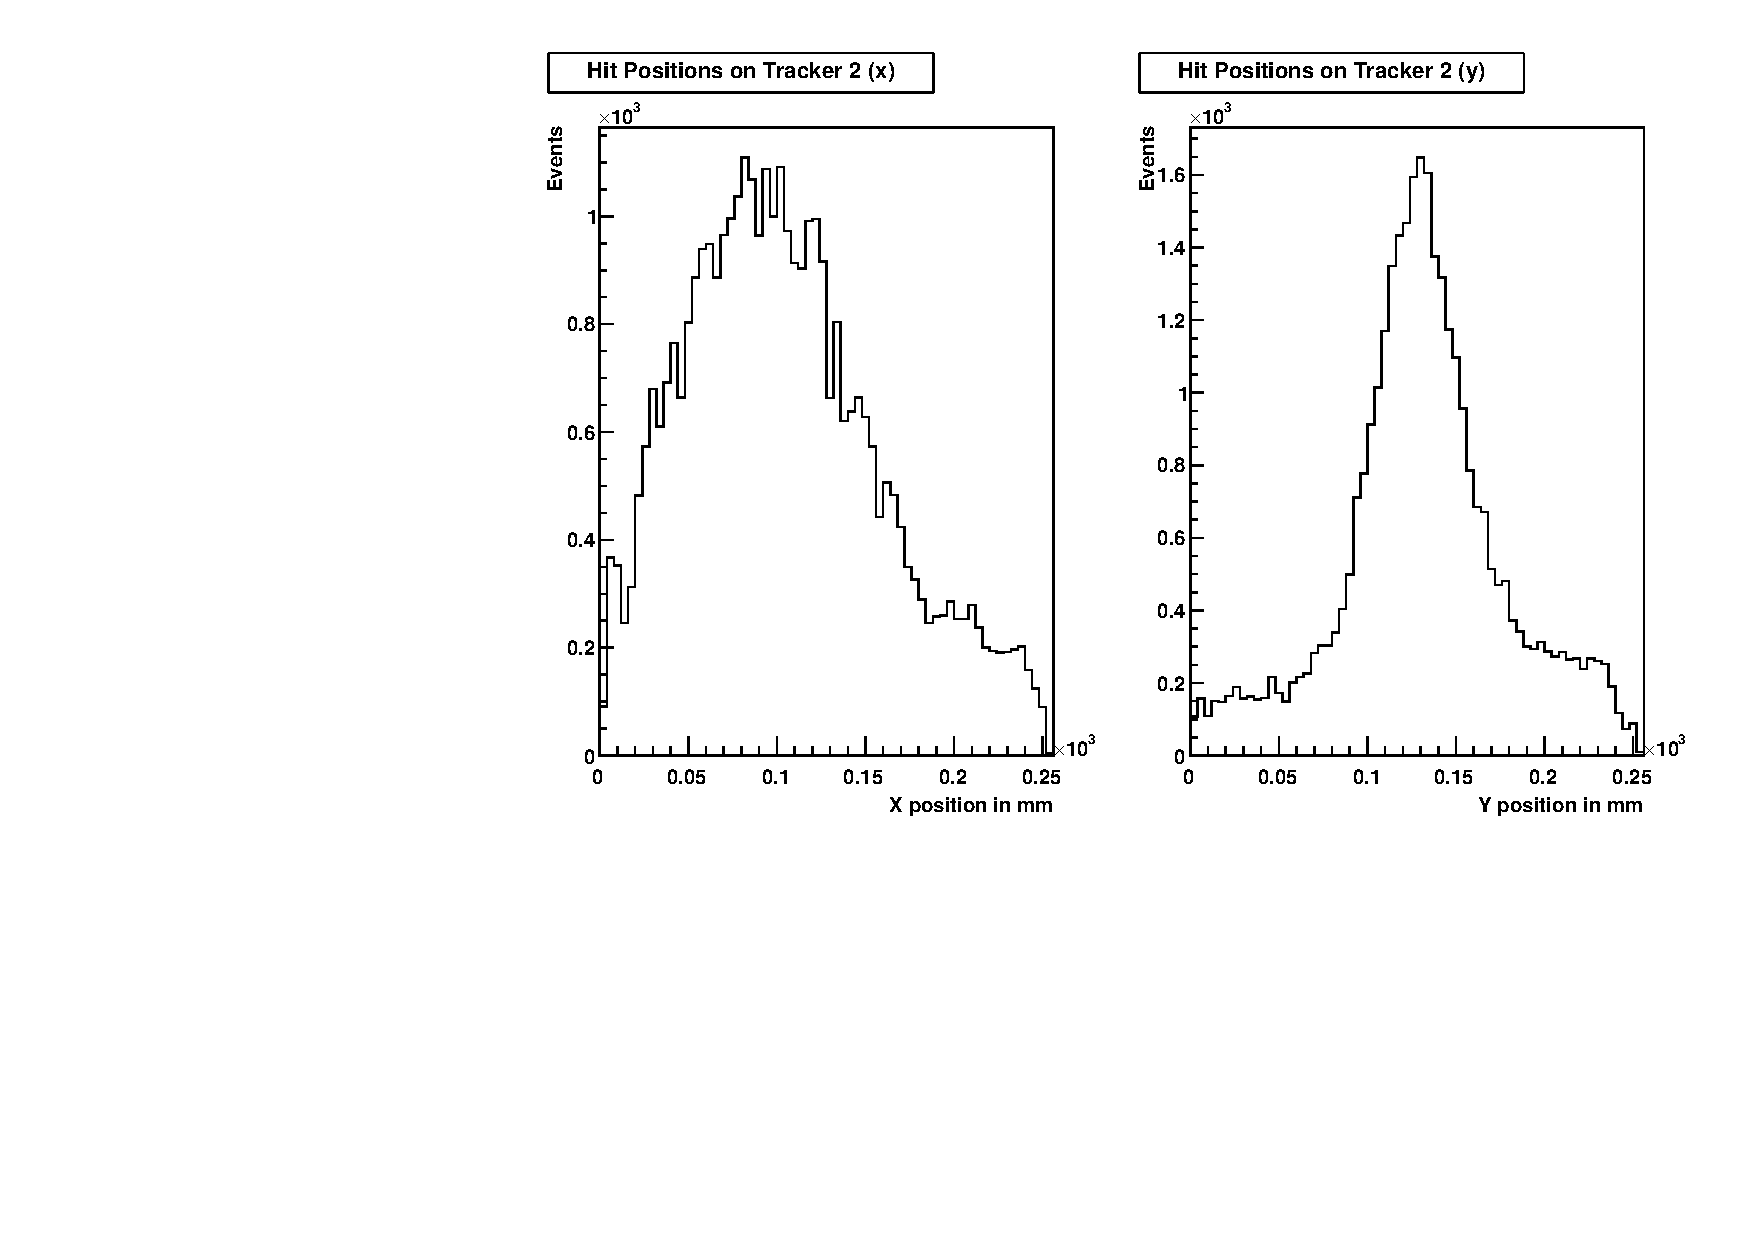
\includegraphics[width=5.1in]{figures/GEM/Tracker2_Hit_position_Run1897.pdf}
% \caption{Tracker 2 hit positions in X direction(left) and Y direction(right)}\label{fig:t2hit}
% \end{figure}
% \begin{figure}[!htbp]
% \centering
% 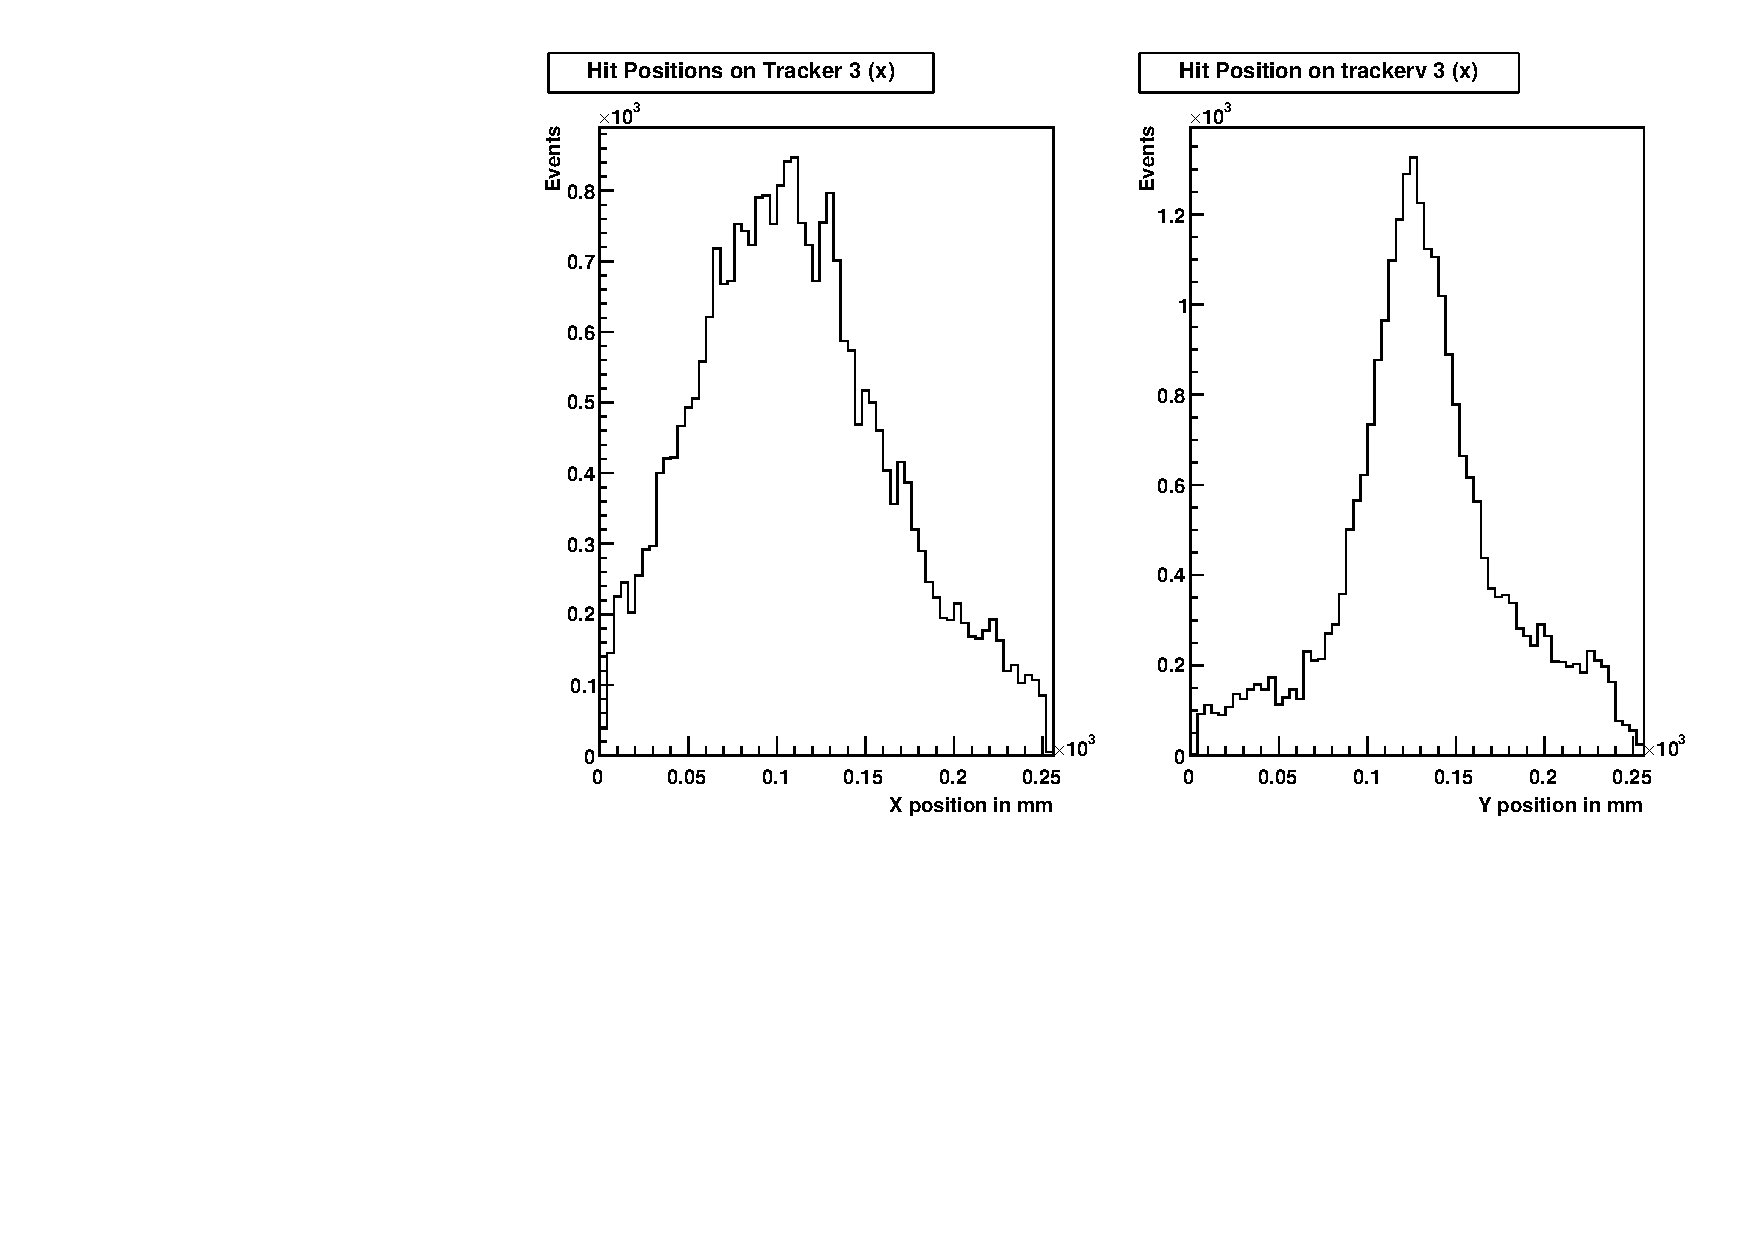
\includegraphics[width=5.1in]{figures/GEM/Tracker3_Hit_position_Run1897.pdf}
% \caption{Tracker 3 hit positions in X direction(left) and Y direction(right)}\label{fig:t3hit}
% \end{figure}
% \begin{figure}[!htbp]
% \centering
% 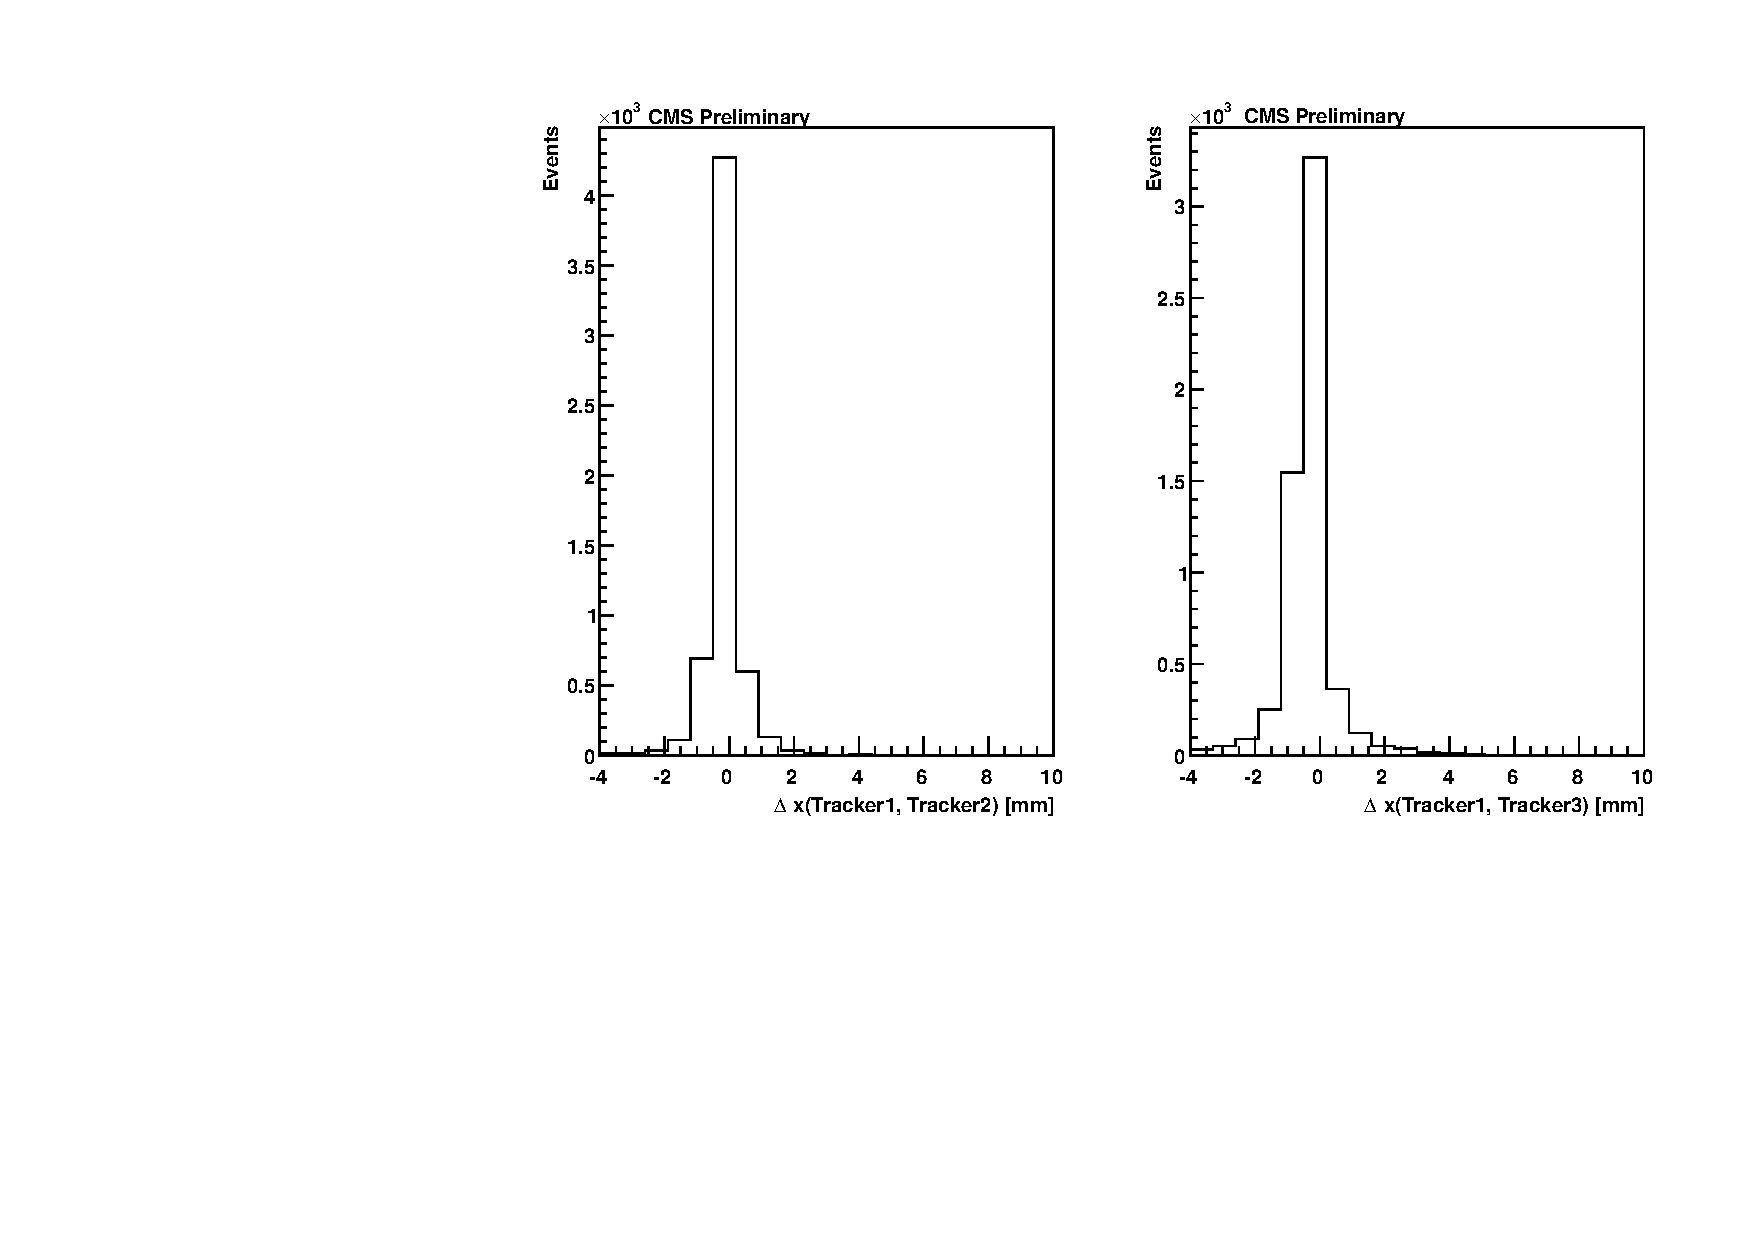
\includegraphics[width=5.1in]{figures/GEM/Offset_1vs23_x_For_Run1897.pdf}
% \caption{X-offset calculated for Tracker2 and Tracker3 w.r.t. the reference Tracker1}\label{fig:Xoff}
% \end{figure}
% \begin{figure}[!htbp]
% \centering
% 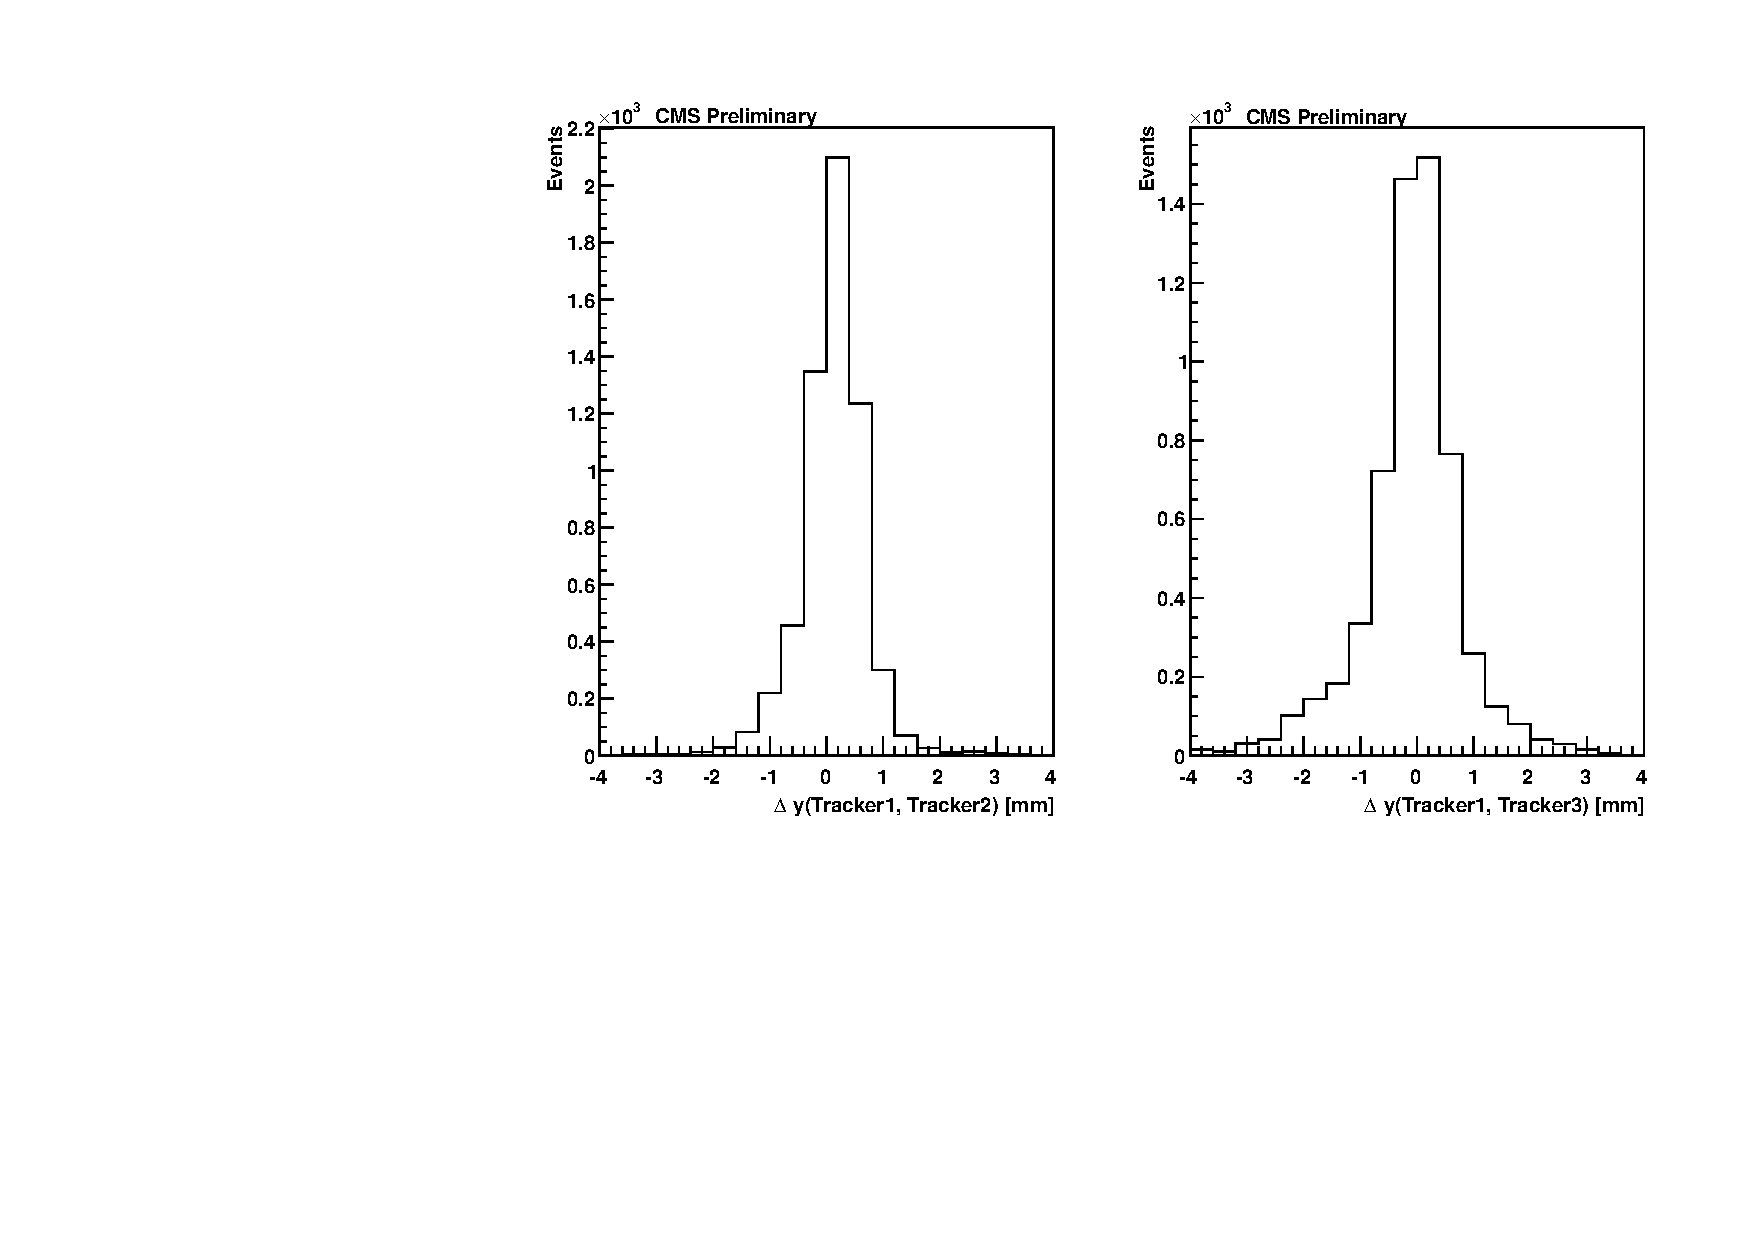
\includegraphics[width=5.1in]{figures/GEM/Offset_For_Tracker1vs23y_Run1897.pdf}
% \caption{Y-offset calculated for Tracker2 and Tracker3 w.r.t. the reference Tracker1}\label{fig:Yoff}
% \end{figure}
% \begin{figure}[!htbp]
% \centering
% 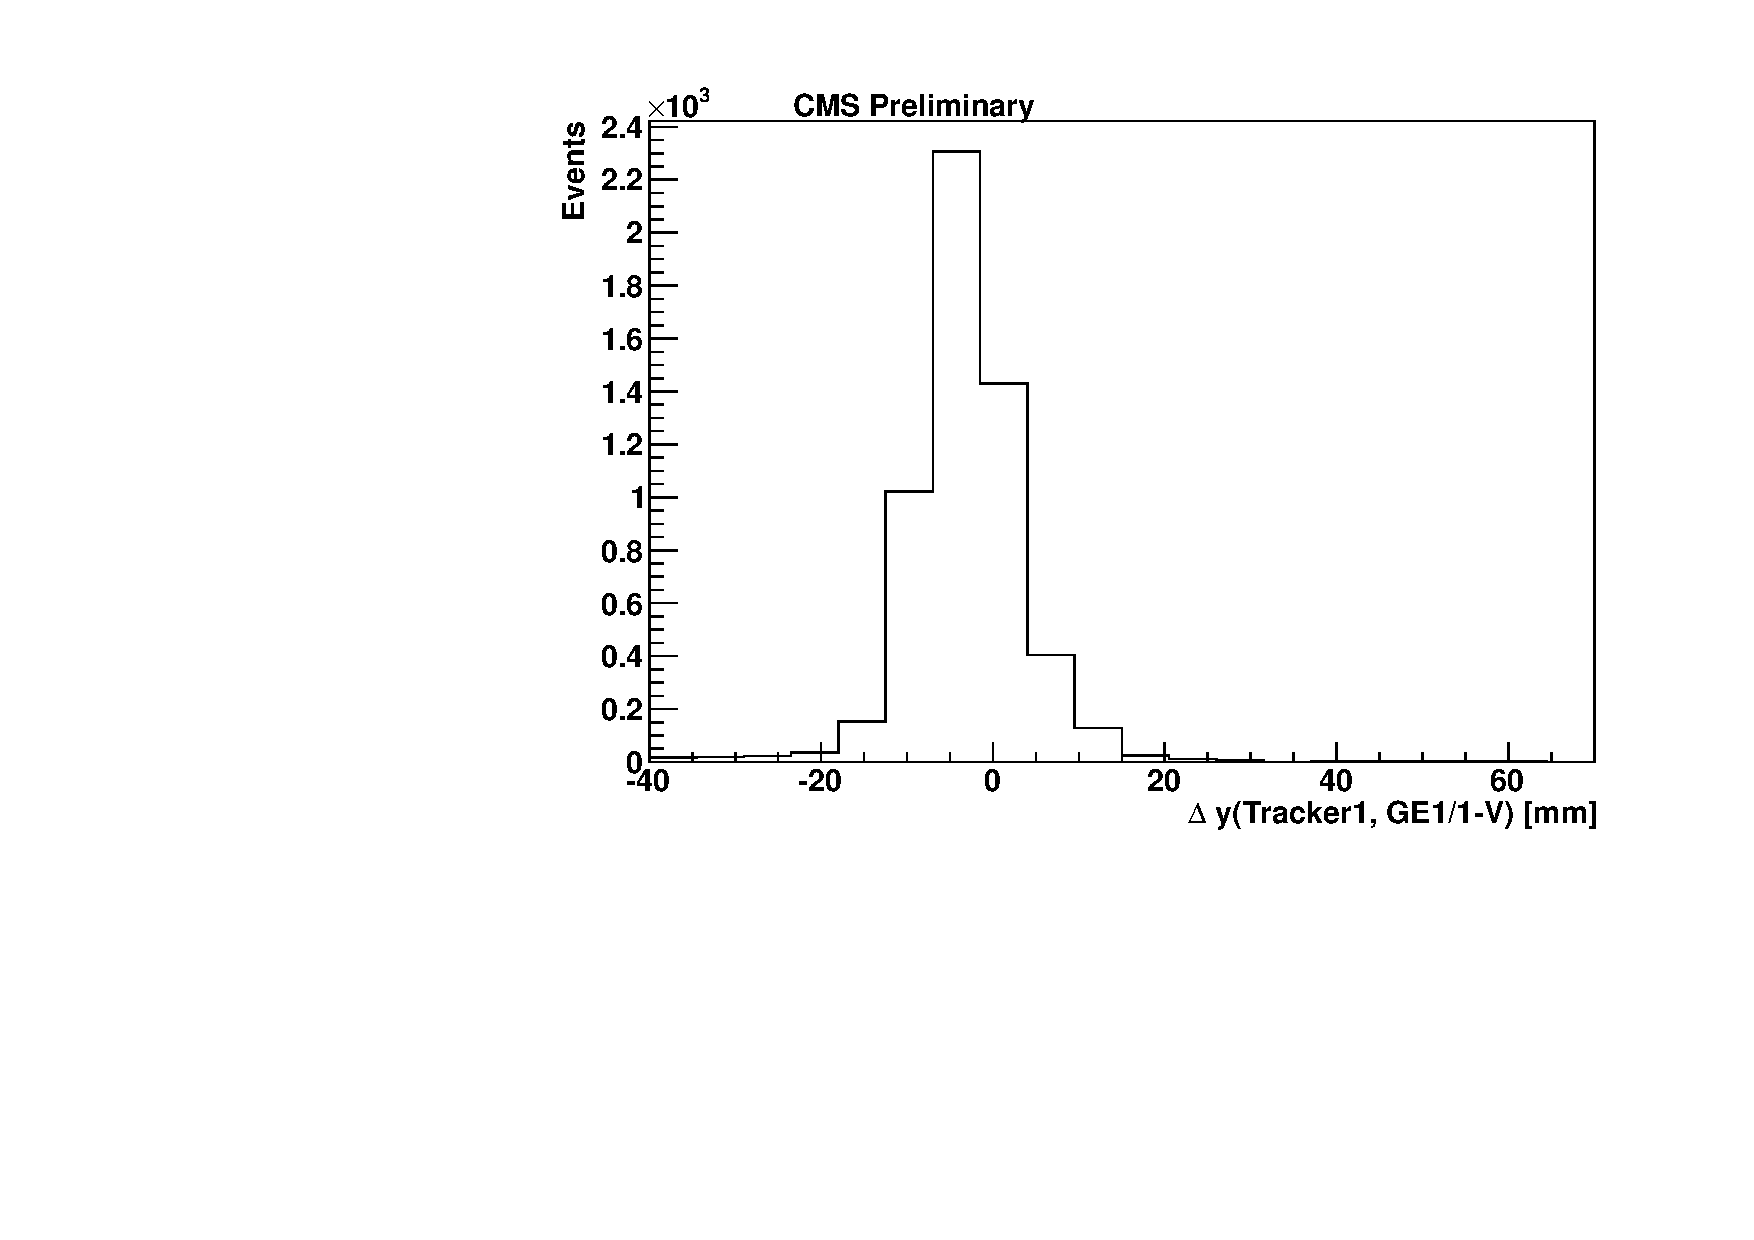
\includegraphics[width=5.1in]{figures/GEM/Offset_Tracker1vsGE11V_X_For_Run1897.pdf}
% \caption{Y-offset calculated for GEM detector GE1/1-V w.r.t. the reference Tracker1}\label{fig:offGEM1}
% \end{figure}
% \begin{figure}[!htbp]
% \centering
% 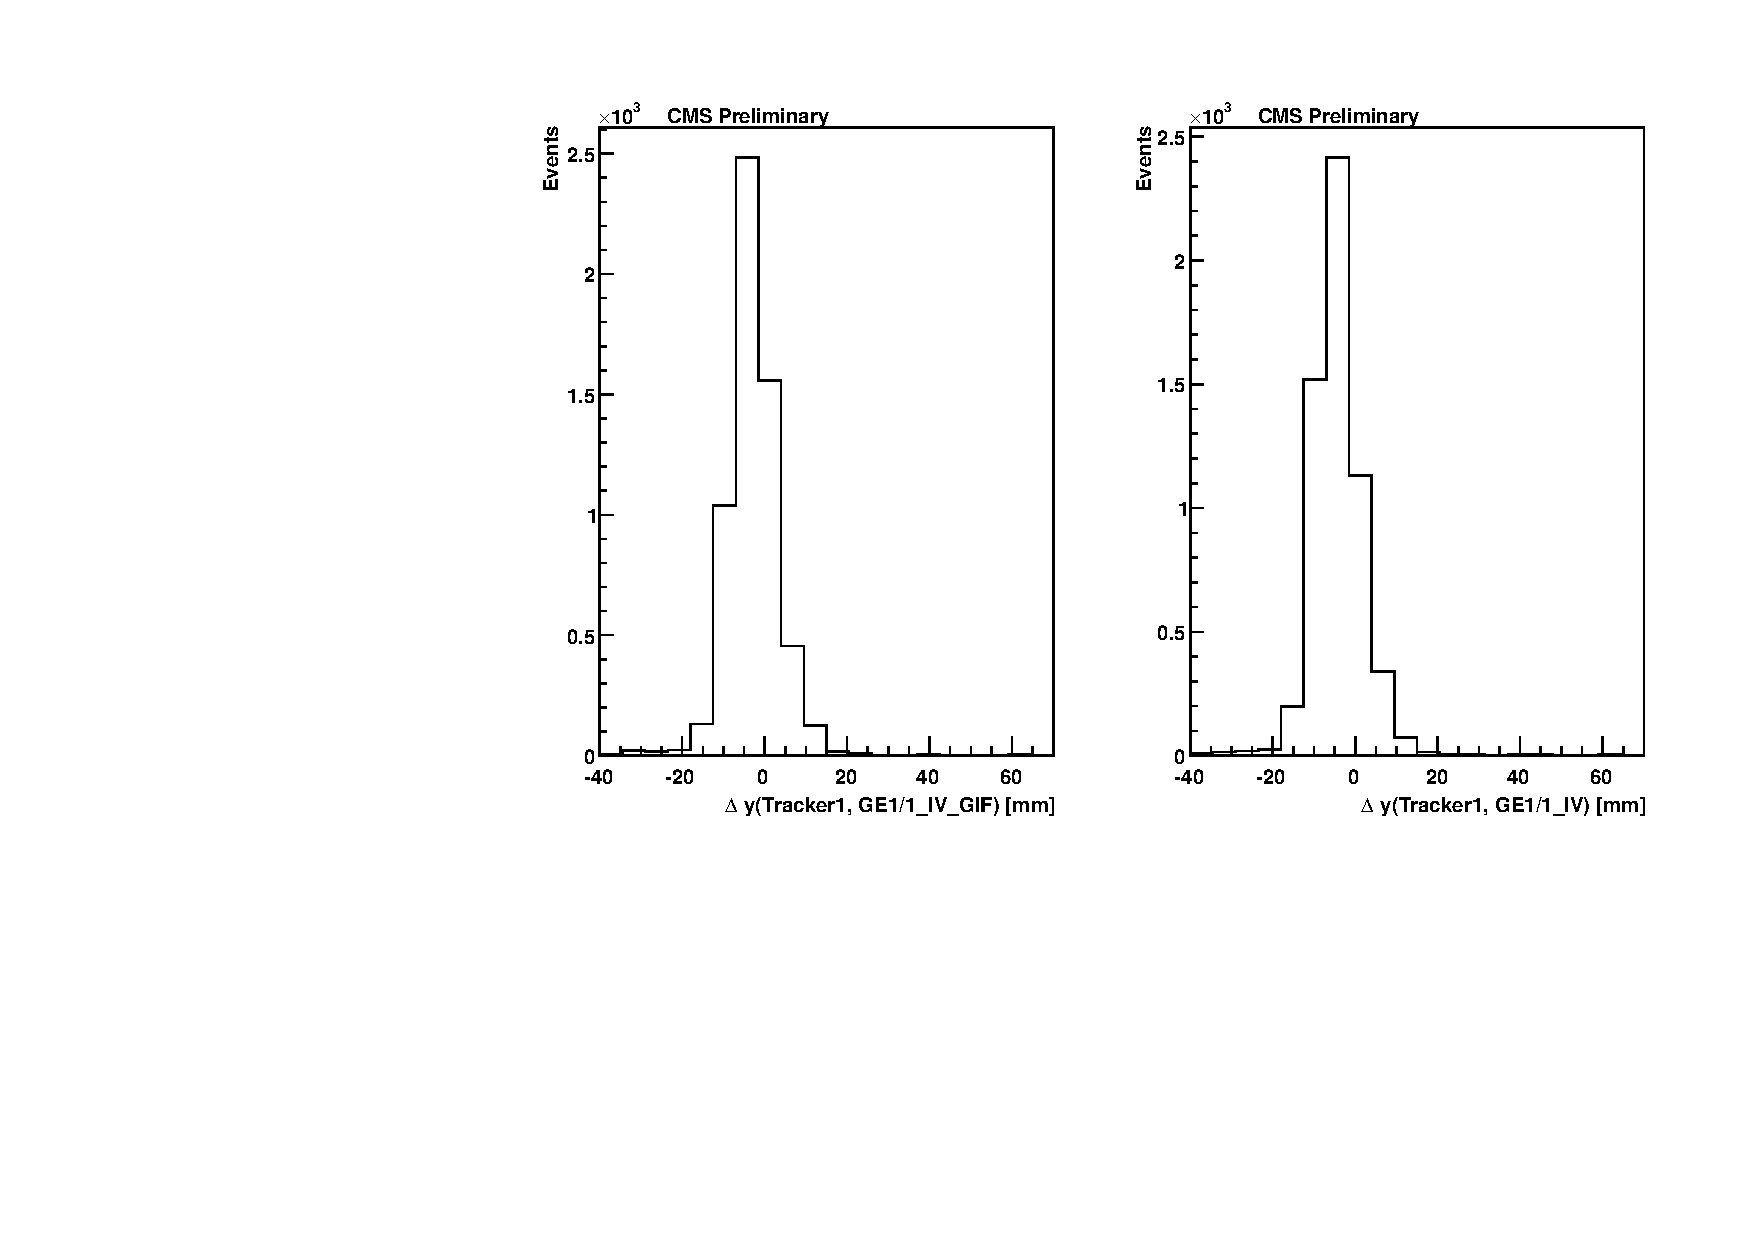
\includegraphics[width=5.1in]{figures/GEM/Offset_1vsGEM_y_For_Run1897.pdf}
% \caption{Y-offset calculated for GEM detectors GE1/1\_IV\_GIF (left) and GE1/1\_IV (right) w.r.t. the reference Tracker1}\label{fig:offGEM2}
% \end{figure}
% \subsubsection{Linear Alignment Using Turbo Software} % (fold)
% \label{ssub:linear_alignment_using_turbo_software}
% A popular alignment method in HEP is based on residual histograms. The basic idea of this method is to extract parameter corrections from the peak (or mean or median) of residual histograms. Histograms of hit residuals are generated and analyzed, and the offsets observed in the histograms are used to adjust the alignment.
% The first tracker, closest to the beam pipe, is taken as a reference detector for alignment. All other detectors are aligned w.r.t. this tracker. Firstly, the three trackers are aligned mutually and then the CMS GEM detectors are aligned w.r.t this tracker system. Hit positions are checked in three trackers. Since there is no magnetic field applied. hence the particle tracks in three trackers are expected to lie on a straight line. Hit positions in three trackers are fitted using a straight line and the residuals (= measured vertical coordinate minus fitted coordinate are histogrammed, separately for each plane. The mean value of the residuals is taken as correction to the vertical plane position of the detectors, and the procedure is repeated iteratively. There are large changes in the first iteration, small changes in the second iteration, and almost no change afterwards.

% % subsubsection linear_alignment_using_turbo_software (end)

\subsubsection{Linear and Rotational Alignment}
To measure the spatial resolution of GEM detectors, these detectors are aligned w.r.t the tracker system.
% \subsubsection{Alignment of Reference Trackers}
The first step in the resolution measurement is an alignment of the three small tracking detectors that have a Cartesian X-Y strip readout.
The trackers are first aligned w.r.t each other in Cartesian coordinates.
The first alignment step is to shift each of the four tracking detectors iteratively in the XY-plane to make their origins match with each other in that plane.
The initial shift parameters are mean values from position distributions in X and Y coordinates. In each iteration, straight lines are fitted to the hits in X and Y.
Residuals are histogrammed for each detector and the residual distributions are fitted with a double-Gaussian function.
Ten percent of the residual mean value of each detector is taken as the shift parameter in the next iteration to avoid overcorrections.
The resulting residual mean values converge quickly towards zero with iterations.
This provides a first coarse alignment.
In a second alignment step, we correct also for relative rotations of the tracking detectors around the beam in the XY-plane.
We again fit straight lines to the hits in X and Y and iterate through a succession of offsets and rotations around the beam axis relative to the first tracking detector until the residual means from the trackers are very close to zero and chi$^2$ of the track fits are minimized.
In each iteration, the detectors are first shifted and then rotated; then new residuals and rotation angles are calculated.
This process is repeated iteratively until the residual means from the track fits becomes less than 0.005 mm.
Figure.~\ref{fig:resvsit} shows the variation of track residuals for three trackers w.r.t the iteration number, with residual converging to lower values with each iteration.
\begin{figure}[!htbp]
\centering
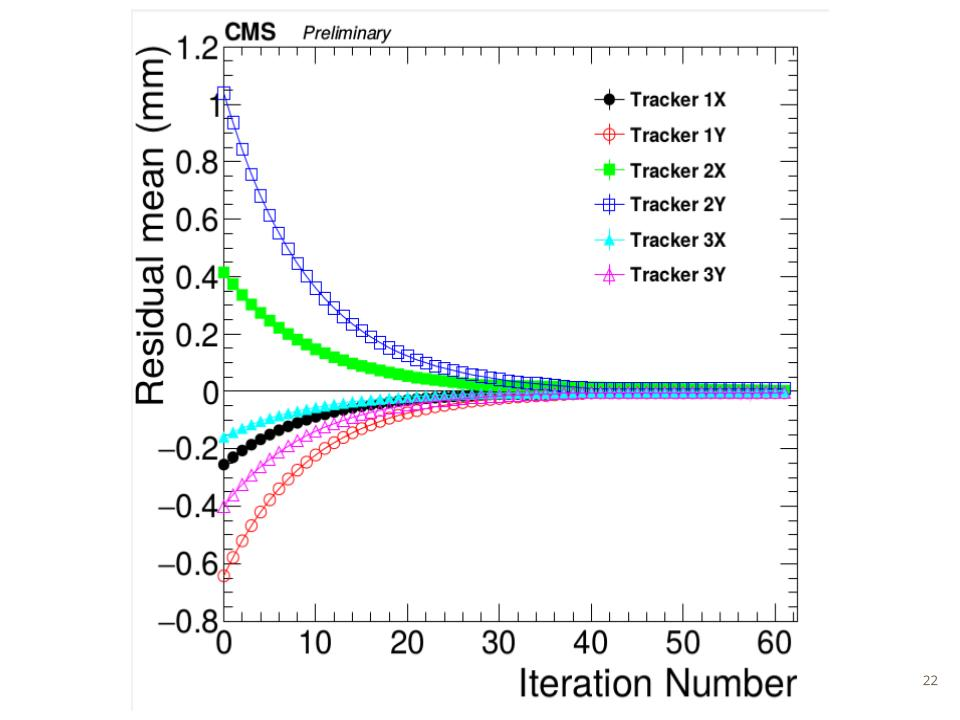
\includegraphics[width=5.1in]{figures/GEM/Tracker_iterative_alignment.jpg}
\caption{Variation of track residuals for three trackers  w.r.t the iteration number}\label{fig:resvsit}
\end{figure}

\subsubsection{Alignment GEM detectors w.r.t Reference Tracker}
After the trackers are aligned w.r.t each other, next step is to align trapezoidal GEM detectors w.r.t the centre of the aligned tracker system.
Twofold iteration loop is used, X offset is kept fixed and iterate over Y offset values with a small fixed step, ranging in a practical phase space. Then X offset is iterated and corresponding iterations are performed with Y offset. For each value of (X offset, Y offset) pair, tracks are linearly fitted in the $\phi$ co-ordinate and the corresponding residuals are noted and used to align the detectors.


\subsubsection{Efficiency Measurement}
Efficiency, $\epsilon$, is one of the most important parameter for the gaseous detectors. Here it is defined as 
\begin{equation}
\epsilon = \frac{N_{GE1/1+Trk}}{N_{Trk}}
\end{equation}
where $N_{Trk}$ is the number of reconstructed events by using a linear fit $y = mx + b$ fit to the tracker hit positions, in the tracker with normalized $\chi^2<10$.
$N_{GE1/1+Trk}$ is the number of reconstructed events for which an actual hit is found in the GE1/1 within $5mm$ of an extra-plotted track.
We are showing here the efficiency as a function of $E_{gain}$, Fig. \ref{Efficiency}. 
\begin{figure}[!htbp]
\centering
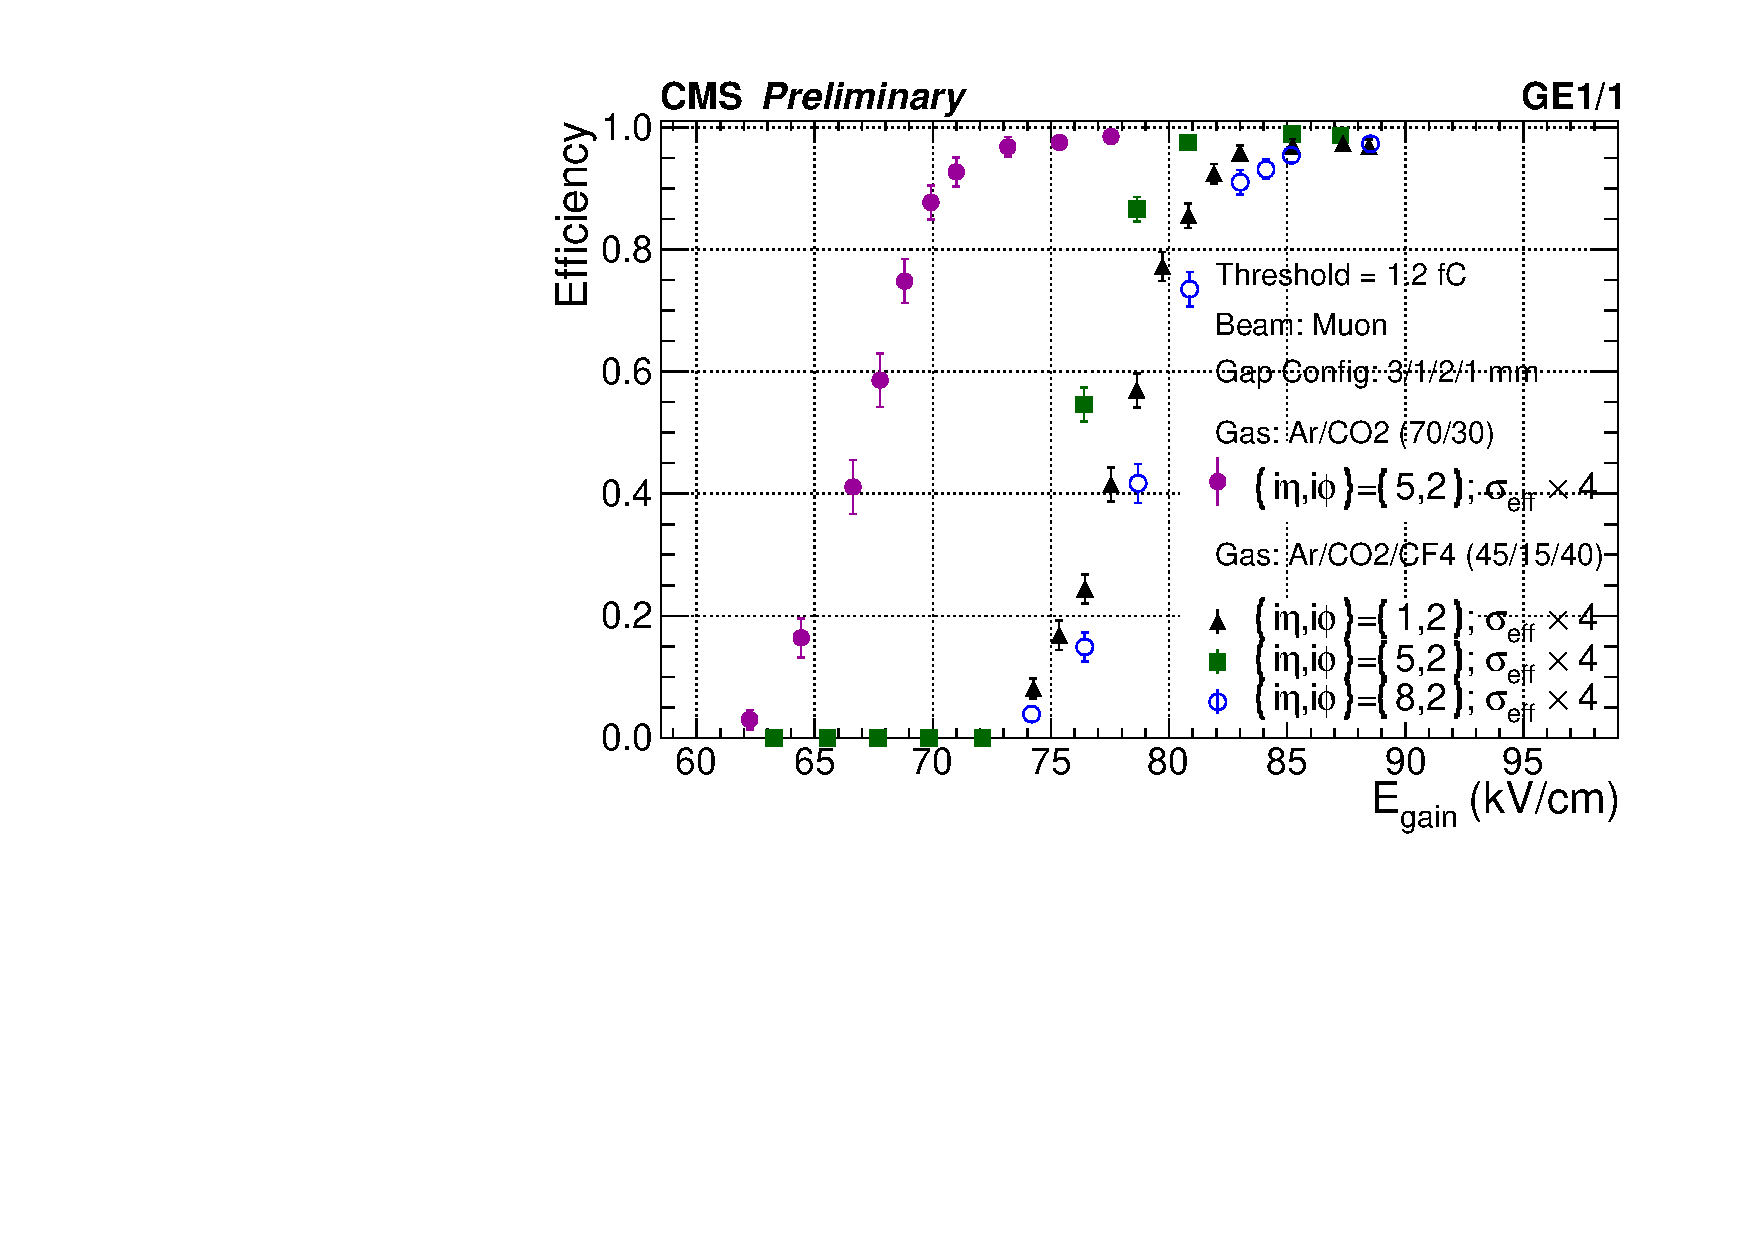
\includegraphics[width=3.5in]{figures/GEM/EfficiencyPlot_wrt_EGain_wError4times_2gas.pdf}
\caption{Efficiency w.r.t. $E_{gain}$ for two different gases and three different $(i\eta,i\phi)$ sectors.}
\label{Efficiency}
\end{figure}
Where $E_{gain}$ is defined as
\begin{equation}
E_{gain} = \frac{I\times R_{avg}^{gap}}{D}
\end{equation}
Where $I$ is current supplied to the HV divider,
      $R_{avg}^{gap}$ is the average gap resistance of GE1/1,
      and D is the thickness of GEM foil.
      Fig. \ref{Efficiency} is showing the efficiency w.r.t. two different gas mixtures $Ar/CO_2$ (70/30) at sector $(i\eta,i\phi)=(5,2)$ and $Ar/CO_2/CF_4$ (45/15/40) scanned at three different sectors $(i\eta,i\phi)=\{(1,2),(5,2),(8,2)\}$. We achieved very good efficiency of $\sim$ 98\% in all cases. While for gas mixture $Ar/CO_2$ the threshold is shifted as compared to the $Ar/CO_2/CF_4$ because at fixed high voltage operating point, the effective gain with $Ar/CO_2$  mixture is approximately one order of magnitude higher than $Ar/CO_2/CF_4$ mixture.
      

\subsubsection{Timing Measurement}
The time resolution of a detector is defined as the minimum gate width necessary on the detection electronics for full efficiency.
Experimentally, the time resolution is the rms of the Gaussian distribution of the time taken by the particle to reach detector from scintillator.
Along with the fast 40MHz (25ns) clock pulse has been used to cope with the LHC bunch crossing. So, the detector time response is modelled as the Gaussian function, $f(t)$, convoluted with a square wave, $g(t)$, having pulse length $f_{clk}=25ns$ to represent discrete sampling. 
%The functions $f(t)$ is given by:
%\begin{equation}
%f(t) = Ae^{-\frac{1}{2}(\frac{t-t_0}{\sigma})^2}
%\end{equation}
%where A is amplitude of Gaussian function, $t_0$  is the mean value of Gaussian, and $\sigma$ is the standard deviation of Gaussian. And, $g(t)$ is given by
%\begin{equation}
%g(t) =
%       \begin{cases}
%               0, & \text{else} \\
%               1, & \text{$-\frac{f_{clk}}{2}<t<\frac{f_{clk}}{2}$}
%       \end{cases}
%\end{equation}
%where, $f_{clk}$ is the length of created 40MHz window.
The convolution of the two functions is
\begin{equation}
(f*g)(t) = A \cdot \sigma \sqrt{\frac{\pi}{2}}\Big(erf\Big(\frac{u_{+}}{\sigma\sqrt{2}}\Big)-erf\Big(\frac{u_{-}}{\sigma\sqrt{2}}\Big)\Big)
\end{equation}
where $A$ is the amplitude of the Gaussian function, $\sigma$ is the standard deviation of Gaussian, and $u_{\pm}= t-t_0\pm\frac{f_{clk}}{2}$. 
We fitted the experimental data with this convoluted function. From, the fit we extract the time resolution of the detector before the convolution. The time resolution as a function of $E_{drift}$ is shown in Fig. \ref{TimeResolution}. The time resolution with $Ar/CO_2$ (70/30) is higher for lower values of $E_{drift}$. However for any given point on the $Ar/CO_2$ curve has a gain approximately one order of magnitude higher gain than the corresponding gain with $Ar/CO_2/CF_4$ (45/15/40).  We are able to reach faster timing at lower gains with the addition of the $CF_4$ and this is important from the point of view of detector safety because this will allow us to operate the detector at lower gains, hence reducing the discharge probability.

\begin{figure}[!htbp]
\centering
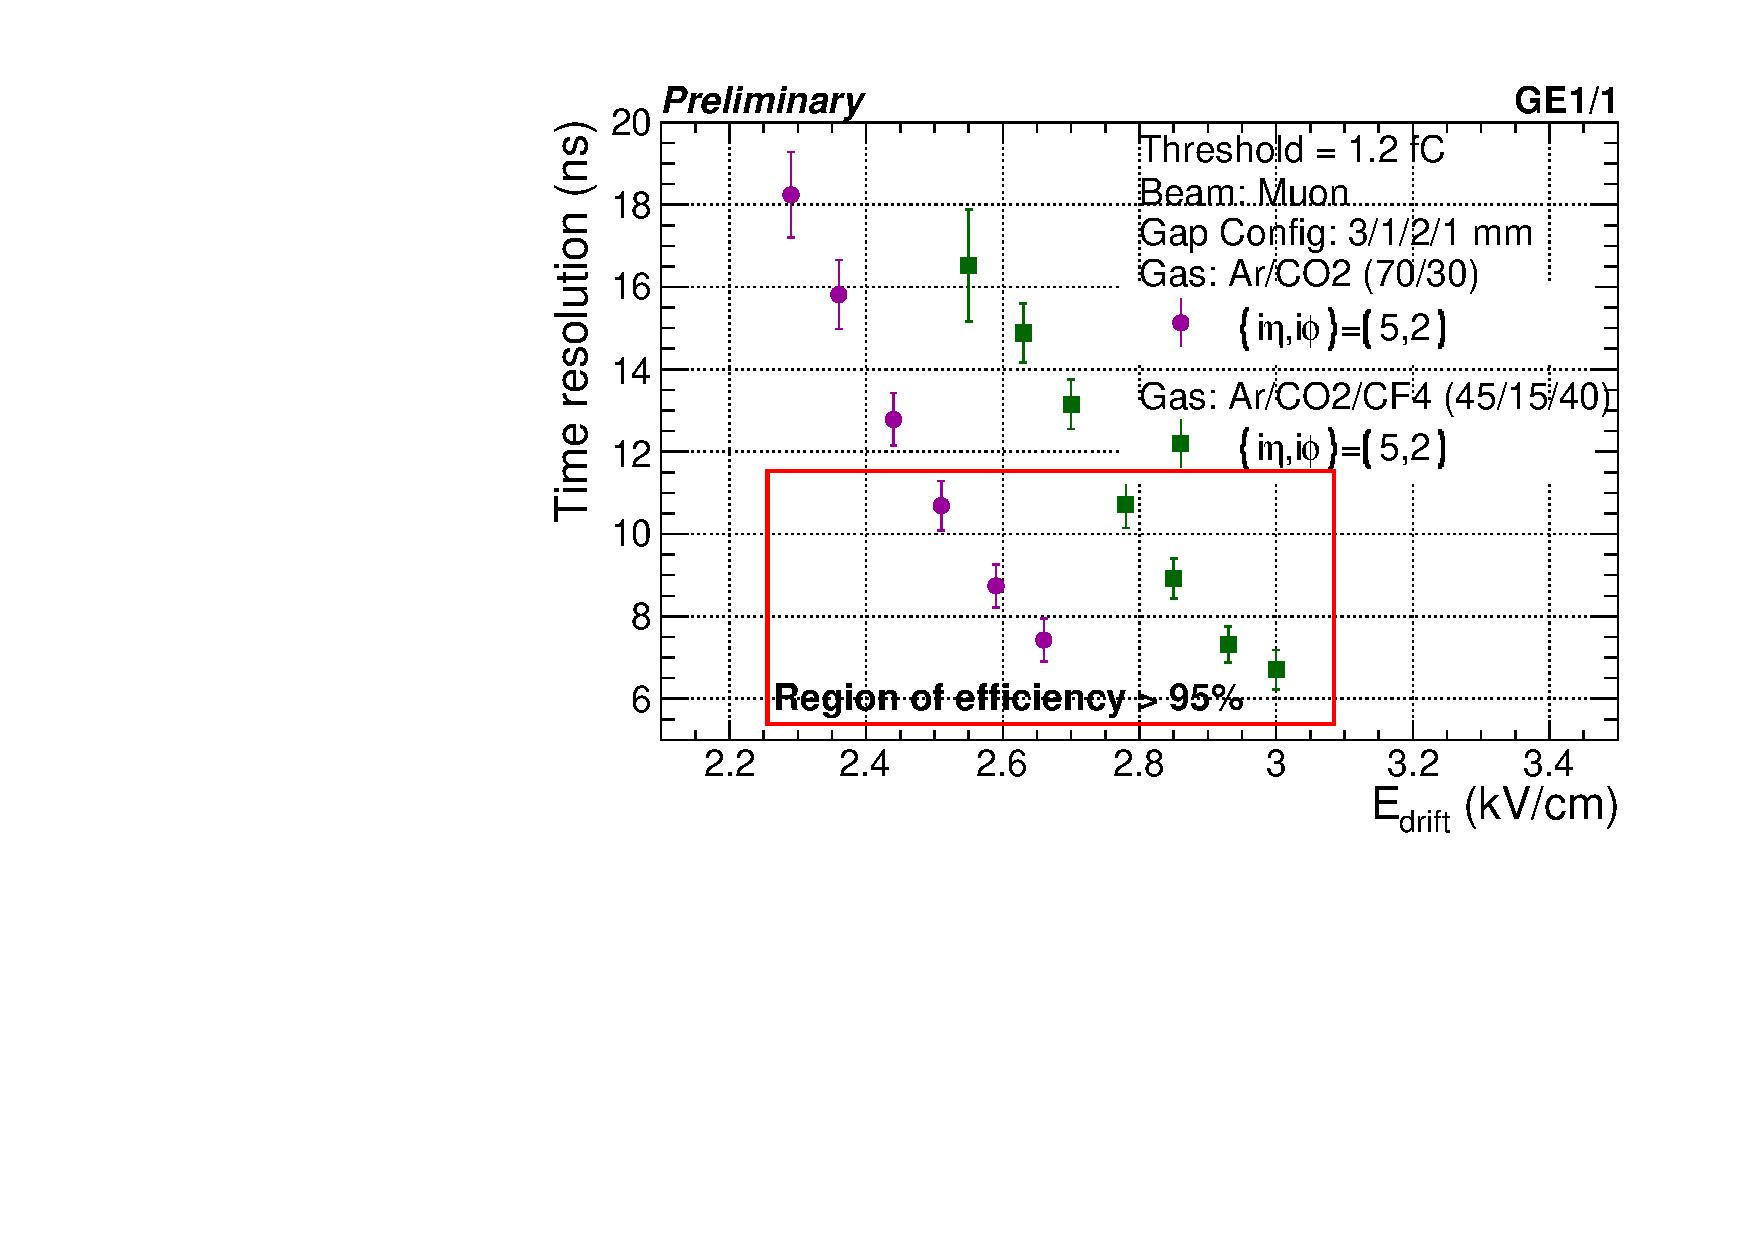
\includegraphics[width=3.5in]{figures/GEM/TimeResolution_wrt_EDrift.pdf}
\caption{Time-resolution w.r.t. $E_{drift}$ for two different gases.}
\label{TimeResolution}
\end{figure}



\subsubsection{Cluster Size Study}

Cluster size is defined as the average number of readout strips sharing charge from ionisation of single charged particles.
To study the cluster size, clusterization algorithm is used. The basis of this algorithm is that we considered clusters if there are one or more continuous strips are fired.
Three golden run ranges are studied with different eta sector are as :\\
\begin{itemize}
\item{Run 1592 - 1646 (i$\eta$, i$\phi$) = (5,2)}
\item{Run 1869 - 1903 (i$\eta$, i$\phi$) = (8,2)}
\item{Run 2065 - 2123 (i$\eta$, i$\phi$) = (1,2)}
\end{itemize}
To fit the cluster size distribution, Poisson function is used that calculates the number of events in specified intervals. Figure~\ref{fig:CSDpoissonfunction} shows the cluster size distribution for different ($\eta$, $\phi$) sector fitted with the Poisson distribution function.
%\begin{itemize}
  \begin{figure}[!htbp]
    \begin{center}
      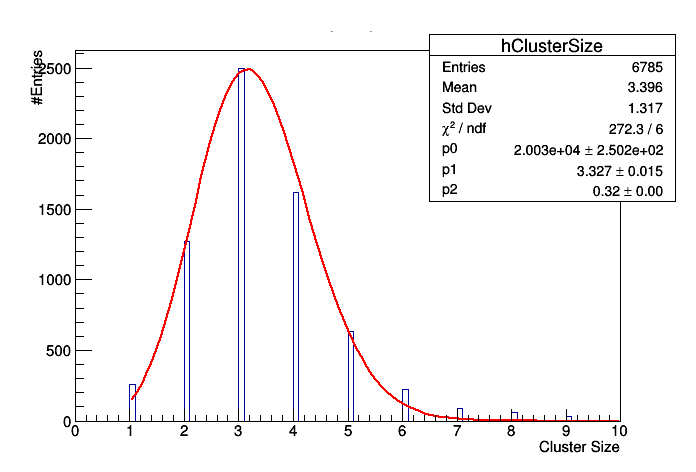
\includegraphics[width=6cm,height=6cm]{figures/GEM/Run1644.png}
      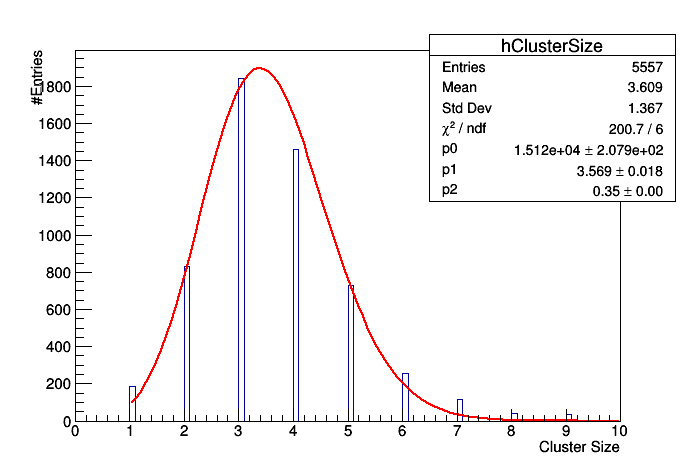
\includegraphics[width=6cm,height=6cm]{figures/GEM/Run1869.png}
      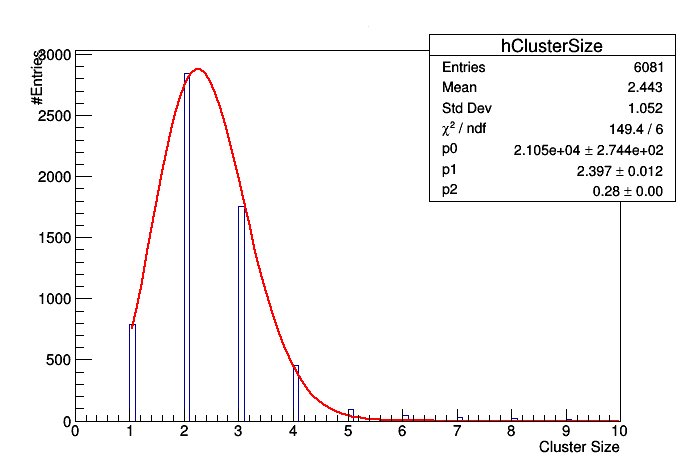
\includegraphics[width=6cm,height=6cm]{figures/GEM/Run2066.png}
    \end{center}
    \caption{Left: Cluster size distribution for Run1644 in ($\eta$, $\phi$) = (5,2), Right: For Run1869 in ($\eta$, $\phi$) = (8,2), Bottom: For Run2066 in ($\eta$, $\phi$ = (1,2)}
    \label{fig:CSDpoissonfunction}
    %    \end{center}
  \end{figure}
  % \end{itemize}
Study for the cluster size is done only for the three above mentioned golden run ranges. Distribution is studied with the different fiducial region (full exposed area of the detector). Figure~\ref{fig:CSDfiducialregion} shows that the cluster size is independent of the fiducial region.
\begin{figure}[!htbp]
    \begin{center}

      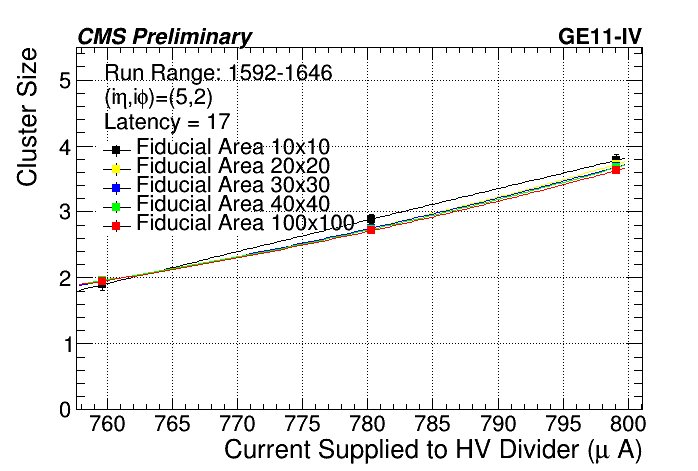
\includegraphics[width=6cm,height=6cm]{figures/GEM/CurrentvsClusterSizeR1592R1646.png}
      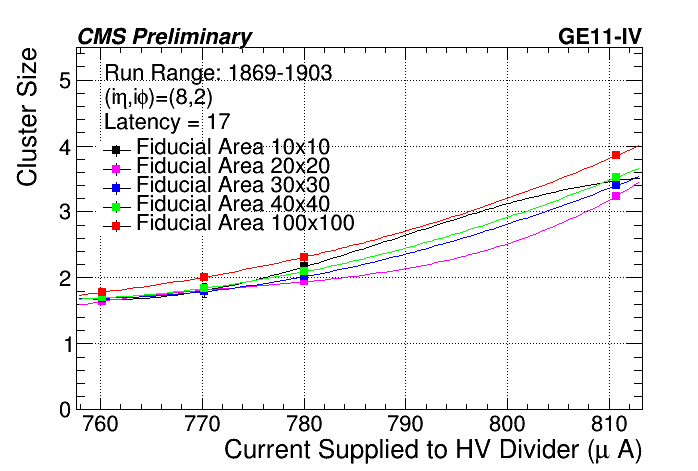
\includegraphics[width=6cm,height=6cm]{figures/GEM/CurrentvsClusterSizeR1869R1903.png}
      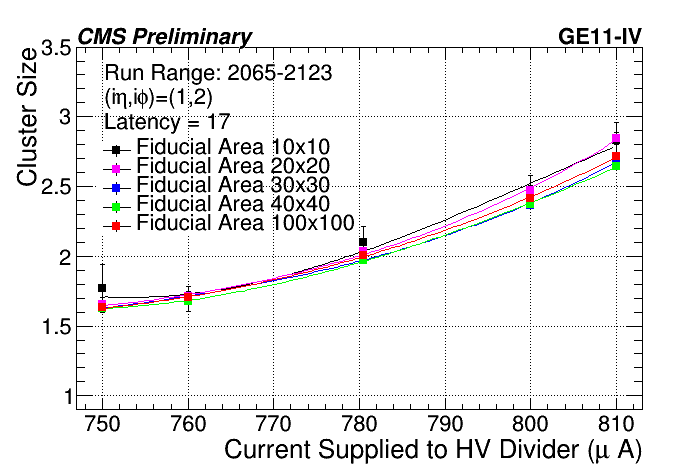
\includegraphics[width=6cm,height=6cm]{figures/GEM/CurrentvsClusterSizeR2065R2123.png}
    \end{center}
    \caption{Cluster size distribution with different fiducial region: Left - Run1592\_R1646 in ($\eta$, $\phi$) = (5,2), Right - Run1869\_R1903 in ($\eta$, $\phi$) = (8,2), Bottom - Run2065\_R2123 in ($\eta$, $\phi$) = (1,2)}
  \label{fig:CSDfiducialregion}
\end{figure}
\begin{figure}[!htbp]
   \begin{center}
     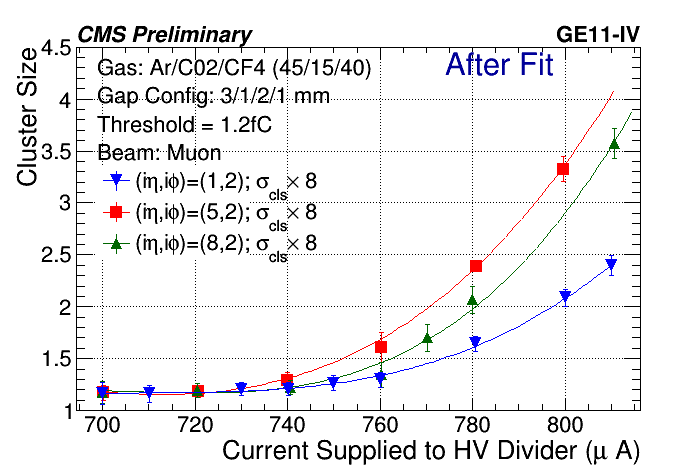
\includegraphics[width=6cm,height=6cm]{figures/GEM/CurrentvsClusterSizeAll3EtaPhi.png}
     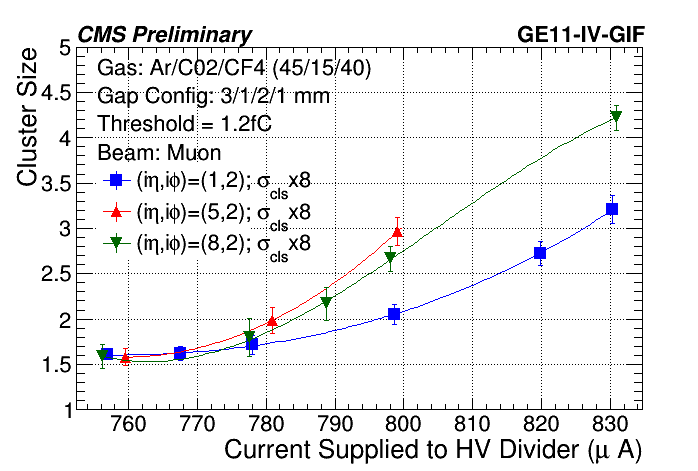
\includegraphics[width=6cm,height=6cm]{figures/GEM/CurrentvsClusterSizeAll3EtaPhiGE11IVGIF.png}
   \end{center}
   \caption{Cluster size distribution: Left - GE1/1-IV, Right - GE1/1-IV-GIF}
   \label{fig:CSDGE1/1}
\end{figure}
Final cluster size study distributions for the GE1/1-IV and GE1/1-IV-GIF (Detector irradiated with Gamma radiations) are plotted with respect to the current supplied to the high voltage divider and shown in Figure~\ref{fig:CSDGE1/1}.
Cluster size is taken with the Poisson fitting function. The cluster size is greater in ($\eta$, $\phi$) = (1,2) region for both the detectors due to the uniformity in readouts channels.
% subsection results (end)

% section gem_for_cms (end)


\section{Fabrication \& Characterization} % (fold)
\label{sec:fabrication_&_characterization}
\subsection{Foil Production}
Through Transfer of Technology (TOT) Micropack signed an agreement for the development of GEM foils in India in collaboration with Indian Institutions. 
After continuous efforts, refining of processes and repeated trials, Micropack has been successful in realizing $10~cm~\times~10~cm$ and $30~cm~\times~30~cm$ GEM foils, meeting the standard dimensional requirements.
Micropack started the production with single mask process as this configuration is the one we are going to use in CMS detector.
But, after several attempts they realized that this is quite challenging so they switched to the double mask process. They quickly succeeded in production of the double-mask GEMs.
It is produced in a similar fashion as at CERN PCB workshop~\cite{DEOLIVEIRA2009}.
The foil used by Micropack was 50 $\mu m$ PI (Apical Type NP) film with 5 $\mu m$ copper coating on both sides.
Figure~\ref{fig:Foil_and_Cone}(a) shows the $10~cm~\times~10~cm$ GEM foil produced by Micropack and the Fig.~\ref{fig:Foil_and_Cone}(b) shows the cross-sectional view of the foil showing the double conical structure.
To qualify these GEM foils as commercially and scientifically reliable, the number of quality control test has to be performed. 
The two main quality control tests are optical test and electrical test. The optical test gives us information about the quality of produced foil like the hole geometry, pitch information and about the defects, if any. 
While the electrical test gives us information about the leakage current, discharge effects, etc.
\begin{figure}[!htbp]
    \centering
    \begin{subfigure}[b]{0.46\textwidth}
        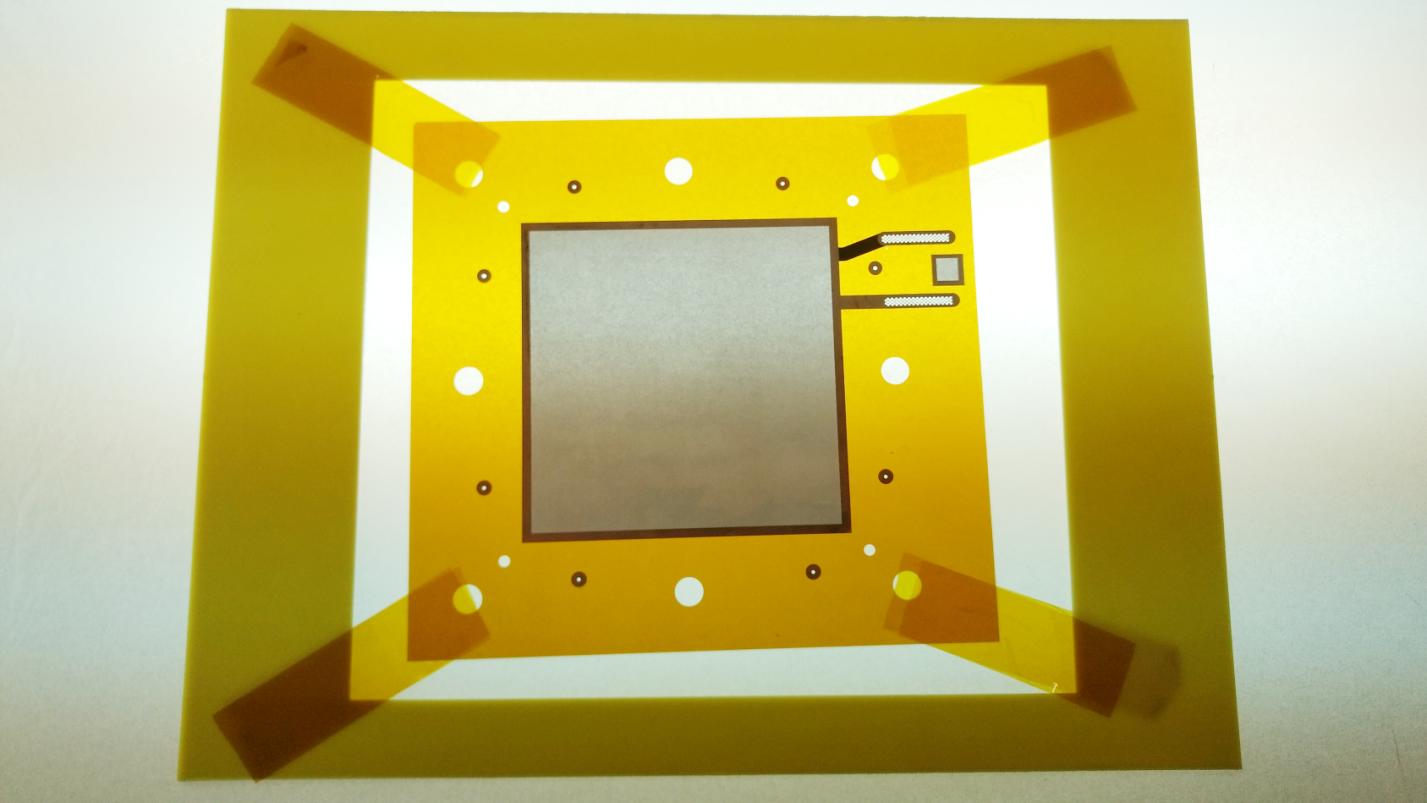
\includegraphics[width=6cm, height=4cm]{figures/GEM/figures/Foil_01.png}\qquad
        \caption{ }
    \end{subfigure}
    \begin{subfigure}[b]{0.46\textwidth}
        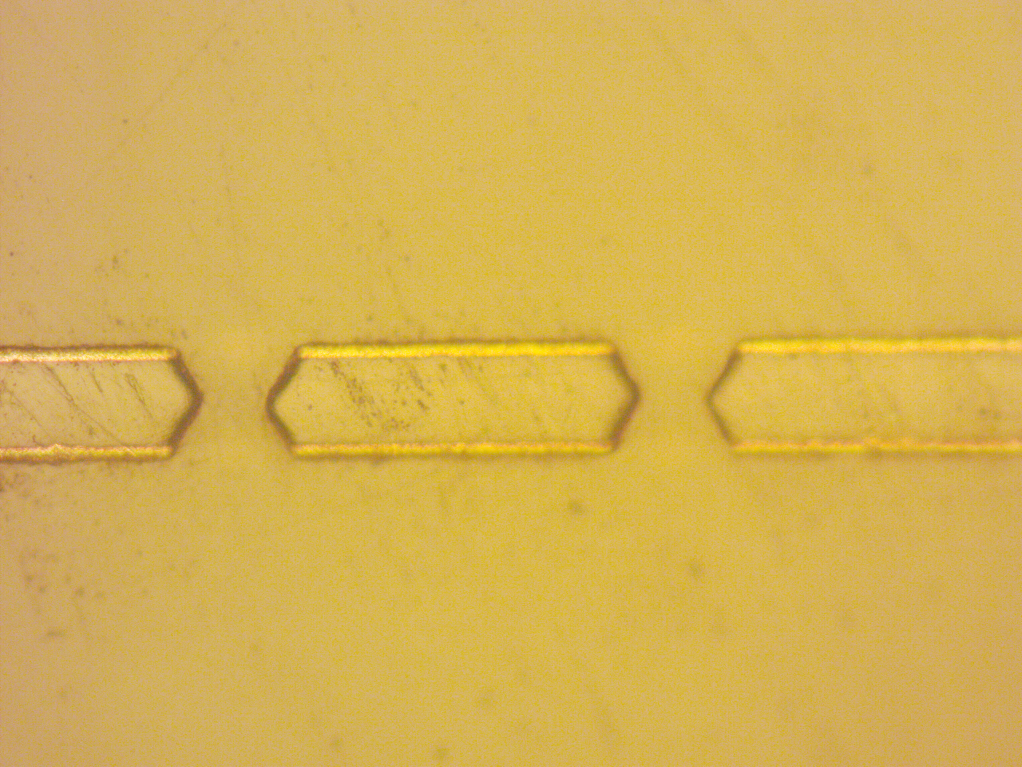
\includegraphics[width=6cm, height=4cm]{figures/GEM/figures/double_cone.png}
        \caption{ }
    \end{subfigure}
   \caption{(a) 10 cm $\times$ 10 cm GEM foil encapsulated in a frame and (b) Cross-sectional view of the foil showing the double cone structure of the engraved holes. } \label{fig:Foil_and_Cone}
\end{figure}

\subsection{Optical Assessment}
GEM performance depends heavily on the quality and parameters of GEM foil like thickness of foil, hole diameter, pitch, and defects like missing holes, un-etched areas, excess-etching, burnt areas, etc. 
To check these defects and to measure the hole-size and pitch several methods was developed using an automated 2D-CCD scanner~\cite{Posik2015, Becker2006}. 
However we used a different technique. We divided the GEM foil into several sectors and captured a high-resolution picture using the AF-S Micro Nikon 40 mm 1:2.8G lens. We used a softbox ($1~m~\times~1~m$) light source for uniform illuminating the GEM foil.
A sketch of the set-up is shown in Fig.~\ref{fig:Optical_Sketch}.
\begin{figure}[!htbp]
    \centering
    %\begin{subfigure}[b]{0.7\textwidth}
        %\includegraphics[width=12cm, height=8cm]{figures/GEM/figures/NIMA_paper_Images001.jpeg}
        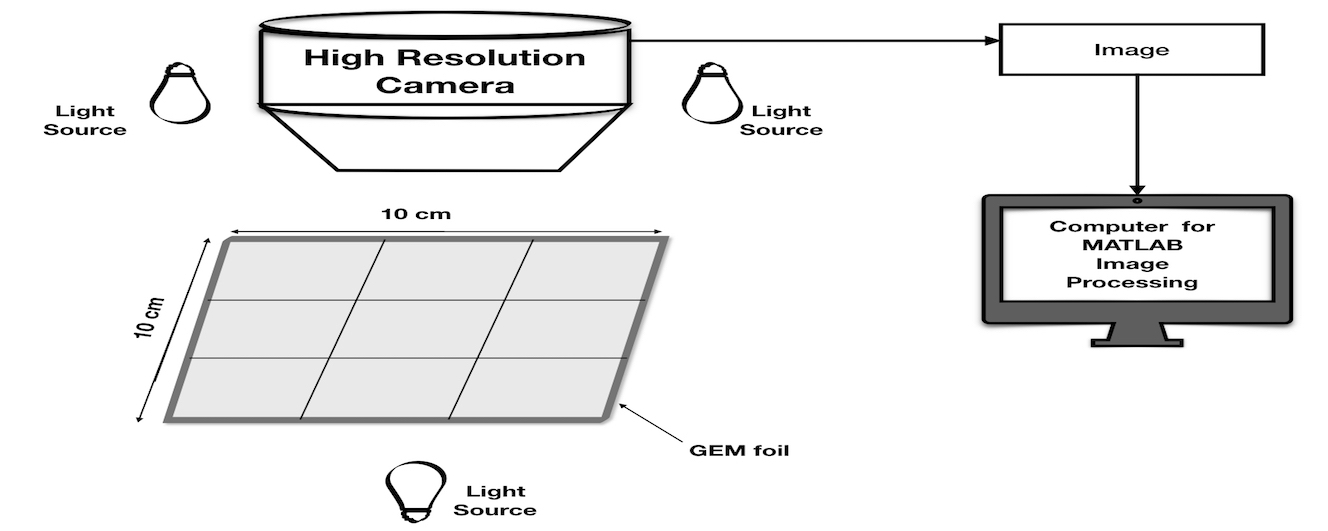
\includegraphics[width=12cm, height=8cm]{figures/GEM/figures/2.jpeg}
        %\includegraphics[width=9cm, height=8cm]{figures/GEM/figures/Optical_Sketch.png}
    %    \caption{ }
    %\end{subfigure}
   \caption{Sketch of the set-up used for the optical measurements.}   \label{fig:Optical_Sketch}
\end{figure}
Fig~\ref{fig:Optical_01} shows the found defects in the considered GEM foil. Also, the measured number of defects is shown in Fig.~\ref{fig:Optical_04}.
\begin{figure}[!htbp]
    \centering
    \begin{subfigure}[b]{0.29\textwidth}
        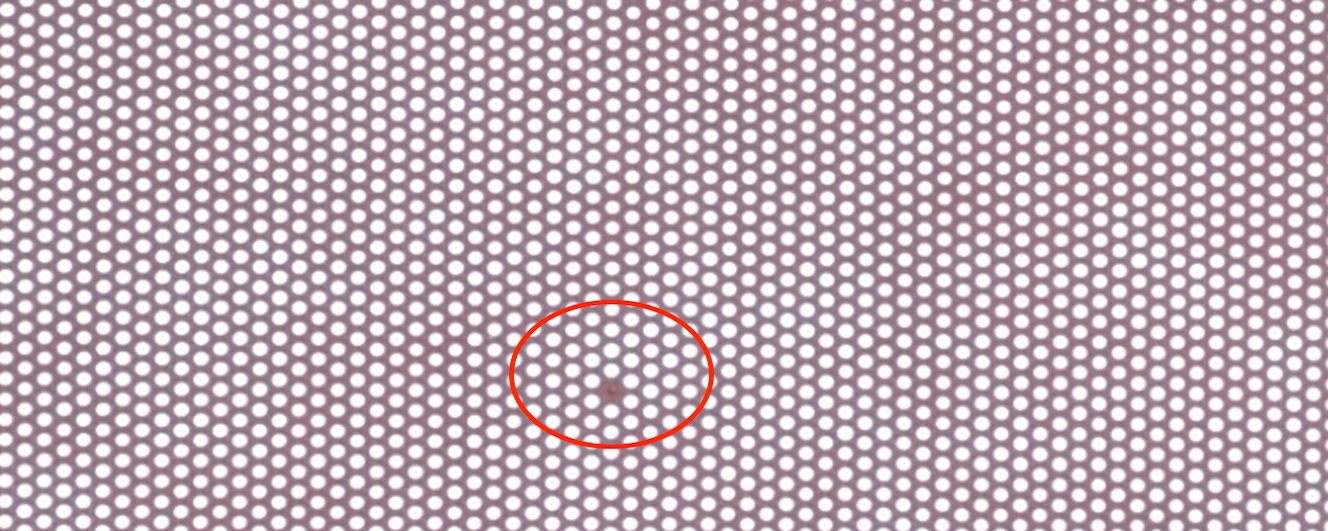
\includegraphics[width=4cm, height=3cm]{figures/GEM/figures/3a.jpg}
        \caption{ }
        \label{fig:O_4a}
    \end{subfigure}
    \begin{subfigure}[b]{0.29\textwidth}
        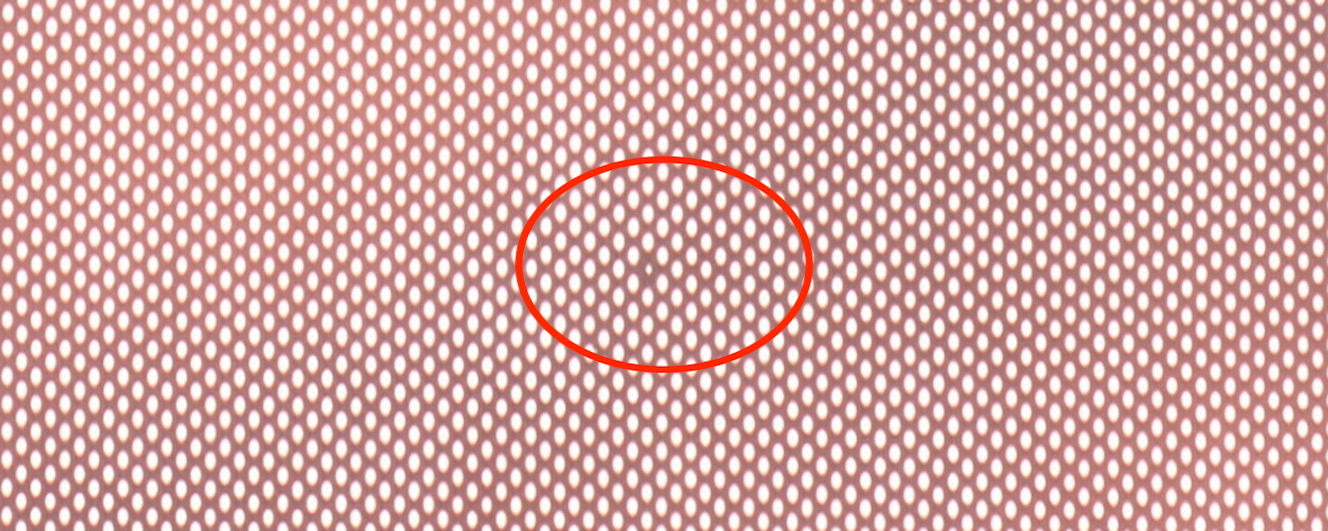
\includegraphics[width=4cm, height=3cm]{figures/GEM/figures/3b.jpg}
        \caption{ }
        \label{fig:O_4b}
    \end{subfigure}
    \centering
    \begin{subfigure}[b]{0.29\textwidth}
        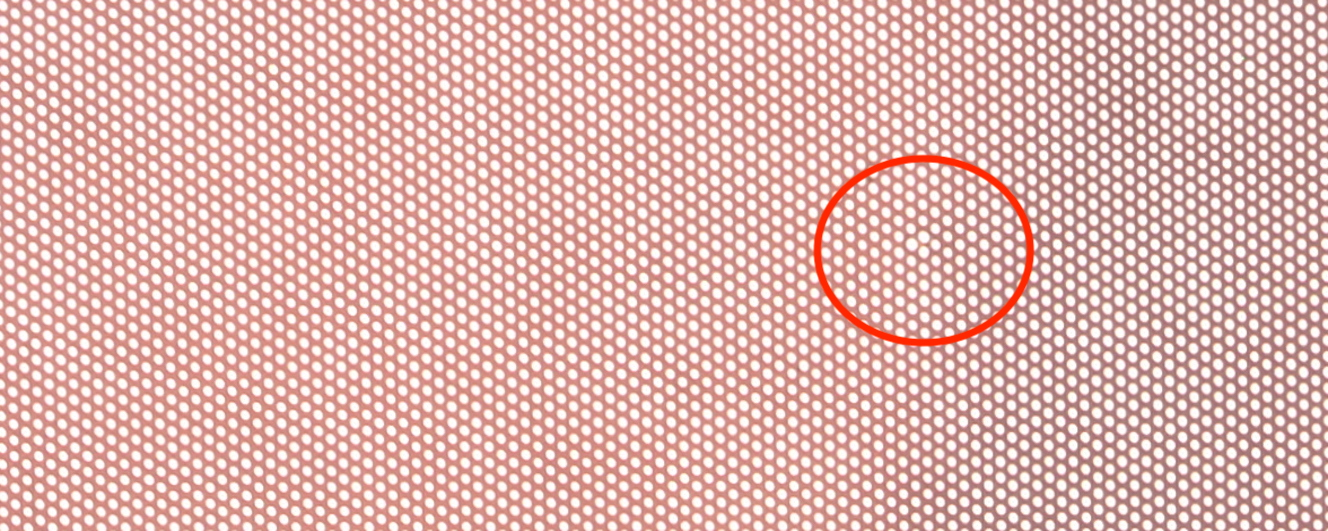
\includegraphics[width=4cm, height=3cm]{figures/GEM/figures/3c.jpg}
        \caption{ }
        \label{fig:O_4c}
    \end{subfigure}
    \centering
    \begin{subfigure}[b]{0.29\textwidth}
        \includegraphics[width=4cm, height=3cm]{figures/GEM/figures/3d.jpg}
        \caption{ }
        \label{fig:O_5a}
    \end{subfigure}
    \centering
    \begin{subfigure}[b]{0.29\textwidth}
        \includegraphics[width=4cm, height=3cm]{figures/GEM/figures/3e.jpg}
        \caption{ }
        \label{fig:O_5b}
    \end{subfigure}
    \centering
    \begin{subfigure}[b]{0.29\textwidth}
        \includegraphics[width=4cm, height=3cm]{figures/GEM/figures/3f.jpg}
        \caption{ }
        \label{fig:O_5c}
    \end{subfigure}
   \caption{Observed imperfections in the foils: (a) Un-etched area, (b) under-size hole, (c) over-size hole (d) missing hole, (e) excess etching and (f) burnt area.} \label{fig:Optical_01}
\end{figure}

% as shown in the Figures \ref{fig:Optical_02} (a) and \ref{fig:Optical_02} (b), respectively. 
% \begin{figure}[!htbp]
%     \centering
%     \begin{subfigure}[b]{0.44\textwidth}
%         \includegraphics[width=5cm, height=4cm]{figures/GEM/figures/O_1b}
%         \caption{ }
%         \label{fig:O_1a}
%     \end{subfigure}
%     \begin{subfigure}[b]{0.44\textwidth}
%         \includegraphics[width=5cm, height=4cm]{figures/GEM/figures/O_1a}
%         \caption{ }
%         \label{fig:O_1b}
%     \end{subfigure}
%    \caption{(a) Outer holes when front light is ON and (b) Inner holes when back light is ON.} \label{fig:Optical_02}
% \end{figure}
%=====================================================================	
%=====================================================================

\begin{figure}[!htbp]
    \centering
    \begin{subfigure}[b]{0.49\textwidth}
        \includegraphics[width=7.6cm, height=5.5cm]{figures/GEM/figures/Apical_Defects.pdf}\qquad
        \caption{ }
        \label{fig:O_9a}
    \end{subfigure}
    \begin{subfigure}[b]{0.49\textwidth}
        \includegraphics[width=7.6cm, height=5.5cm]{figures/GEM/figures/CopperDefects.pdf}
        \caption{ }
        \label{fig:O_9b}
    \end{subfigure}
   \caption{Number of defects seen in (a) Insulator (Apical Type NP) and (b) Copper, for one of the 10 cm $\times$ 10 cm foil.} \label{fig:Optical_04}
\end{figure}

%=====================================================================

\subsection{Electrical Assessment}
The production quality of GEM foils can be quantified through optical and electrical tests. The optical test gives the information regarding the hole geometry and pitch related information whereas electrical test provides the parameters about the efficacy of the foils and hence is important in determining the quality of GEM foils. 
Electrical properties of the GEM foils were discerned by measuring its leakage current extended over a period of time after proper cleaning using adhesive roller.\tabularnewline
We divide electrical tests mainly in two types, quality control short or fast (QC fast) and quality control long (QC long) as per the CERN standards of quality control classification~\cite{Abbaneo2015}, which requires these two tests to be done in order to qualify these foils. 
The difference between QC fast and QC long lies in applying voltage for shorter or longer periods of time respectively, and monitoring the current. 
The other difference being that the QC fast gives the preliminary idea of leakage current or electrical connectivity of the foil but for more detailed study, QC long provides the behaviour of the foil at high voltages in terms of information regarding the actual leakage current and the number of discharges, if any, for the reasonably longer duration of time. 
Here, both the tests have been performed; the electrical connectivity of the foils by QC fast method has been done with insulation tester MIT Megger 420 \cite{twelve}. Using this test, we established that the foils have good electrical connectivity.
\begin{figure}[!htbp]
    \centering
    %\begin{subfigure}[b]{0.7\textwidth}
        \includegraphics[width=12cm,height=8cm]{figures/GEM/figures/10.jpeg}
        %\includegraphics[width=12.0cm, height=9.0cm]{figures/GEM/figures/Electrical_Sketch.png}
    %    \caption{ }
        %\label{fig:Setup}
    %\end{subfigure}
   \caption{Sketch of the set-up used for the measurement of leakage current.} \label{fig:Cleaning_Measurement}
\end{figure}
%=====================================================================
\begin{figure}[!htbp]
    \centering
    \begin{subfigure}[b]{0.5\textwidth}
        %\includegraphics[width=7.5cm, height=5.5cm]{Indian_foils_H20.pdf}
        \includegraphics[width=7.5cm, height=5.5cm]{figures/GEM/figures/Fig_11(a).pdf}
        \caption{ }
        \label{fig:Indian_foils_H20}
    \end{subfigure}
    \begin{subfigure}[b]{0.46\textwidth}
        %\includegraphics[width=7.5cm, height=5.5cm]{CERN_foils.pdf} 
        \includegraphics[width=7.5cm, height=5.5cm]{figures/GEM/figures/Fig_11(b).pdf} 
        \caption{ }
        \label{fig:CERN_foils}
    \end{subfigure}
   \caption{Leakage Current of (a) Micropack Foils and (b) CERN Foils, at an average temperature of T=27$^{\circ}$C and relative humidity equal to 20\%.} \label{fig:L_01}
\end{figure}
%=====================================================================
%\begin{figure}[!htbp]
%    \centering
%    \begin{subfigure}[b]{0.75\textwidth}
%        \includegraphics[width=10cm, height=7cm]{Combined_foils_H20.pdf}
%        %\caption{ }
%        %\label{fig:Combined_foils_H20}
%    \end{subfigure}
%   \caption{Comparison of Leakage Currents between Micropack and CERN foils taken at different voltages.} \label{fig:Combined_foils_H20}
%\end{figure}
%=====================================================================

For the better precision in the current measurement, Keithley Electrometer 6517B \cite{thirteen} has been used. 
The measurement set-up consists of a bare GEM foil connected to Keithley 6517B pico-ammeter interfaced with a computer via a GPIB interface and the LabView program was used to record the measurements as shown in the Figure \ref{fig:Cleaning_Measurement}. The current measurement range was set from 0 to 200 nA, with an accuracy of $\pm$0.2 $\%$.
The leakage current thus measured as a function of applied voltage is shown in Figure \ref{fig:L_01} (a) for the Micropack foils.
For comparison, the same measurement were also done for foils procured from CERN and the results are shown in the Figure \ref{fig:L_01} (b).  
%Figure \ref{fig:Combined_foils_H20} shows the comparison of leakage current between Micropack and CERN foils as a function of applied voltage. 
The Micropack and the CERN foils were found to show similar results under similar ambient conditions.
However, as the humidity escalates, the leakage current in CERN foils increases more rapidly compared to the Micropack foils.
The maximum current of 12 nA and 25 nA at an applied voltage of 550V, corresponding to the humidity of 40\% has been observed in Micropack and CERN foils respectively. Figure \ref{fig:LvH} shows the leakage current for various applied voltages under different ambient conditions.
From the Figure \ref{fig:LvH}, it can be fairly concluded that humidity does have drastic effects on the leakage current measurement.
Therefore, the current was also measured in nitrogen environment. Since, Nitrogen is the contamination free standard medium as it is relatively inert and neither reacts with stored materials nor carries moisture.
By slowly percolating nitrogen gas into the test enclosure, which in our case was a Plexiglass enclosure in which nitrogen gas was continuously flowing, moisture-laden air was purged out and the current was measured. All the foils showed a current less than 1 nA.
\begin{figure}[!htbp]
	\centering
	\includegraphics[width=0.45\textwidth]{figures/GEM/megger.png}
	\caption{caption}
	\label{fig:label}
\end{figure}
All the measurements were carried out in the clean room of class 100 installed with a KANOMAX dust particle counter Model 3887 \cite{fourteen} which monitors the particle count. Humidity was controlled by dehumidifier installed in the clean room.
The QC long test of the GEM foils were performed by placing foils in a Plexiglass enclosure. After flowing nitrogen continuously for more than two hours, the leakage current was measured in each foil at different voltages in steps of 50V starting from 450V and going up until 600V for time intervals nearly equal to 700s.
At 600V, at most two discharges were seen during the time period of around 700s. The corresponding results are shown in Figure \ref{fig:QC_Long_01}. Similar results were obtained for both other foils as shown in Figure \ref{fig:QC_Long_02}.

% section fabrication_&_characterization (end)





% \end{document}



% \section{Summary \& Outlook}
% At the test beam facility at CERN, we studied the efficiency and time response of the GE1/1 detector with the exposure of muon beam. We were able to get very good efficiency $\sim$ 98\% and time resolution $\sim$ 7ns in case of both gas mixtures $Ar/CO_2$ (70/30) and $Ar/CO_2/CF_4$ (45/15/40). In this test beam campaign it was shown that we can operate GEM detectors without using $CF_4$, while keeping same efficiency and timing resolution as with gas mixture $Ar/CO_2/CF_4$.


%=====================================================================
% \section {Conclusion}
% GEM foils were produced for the first time in India under the TOT agreement between Micropack Pvt. Ltd. and CERN. Micropack started the preparations for the GEM foil production in India. The first few attempts saw many deviations from the required quality. With further improvements in etching technology and several rounds of iterations, Micropack finally produced a batch of foils which appeared fine from visual inspection and preliminary checks. However, before these foils could be declared fit for applications and technology as reliable, we had to perform the desired quality assessment and characterization for these foils. For this purpose, we performed optical and electrical tests to check the reliability and usability of the foils. Optical tests reveal that the holes are quite uniform with inner and outer diameters of 49.9 $\pm$ 1.6 $\mu$m and 70.01 $\pm$ 2.02 $\mu$m respectively. Here, the quoted errors are the Gaussian one sigma uncertainty on diameter distributions. A current of less than 1 nA has been observed in dry nitrogen environment from electrical measurements and were in agreement with CERN foils. The measured optical and electrical properties of Micropack foils were found to reflect the desired parameters and are at par with the double mask foils produced at CERN. With the successful production of 10 cm $\times$ 10 cm double-mask GEM foils, Micropack has already extended their infrastructure to handle single-mask technology so that larger foils can be produced in order to ease the commercialization of large area GEM foils.

% chapter gas_electron_multiplier (end)